%!TEX root = ../../report.tex
\chapter{Mechatronic design} % (fold)
\label{cha:design}
Designing a bipedal is a complex task that has been subdivided and analyzed in the chapter \ref{cha:analysis}.
From those results the design of RuBi can be broken down into three pieces: electronics, mechanics and software.
When designing from a holistic point of view, this three combined give a positive synergy which is the burden of this chapter.
The first of the three sections starts with the design of the electronics: from the selection of the motors based on \ref{sec:joints} and \ref{cha:mathematical_model} to the custom interfaces developed in order to reduce the weight.
Continues with the mechanical design that gathers all the constraints got from the sections \ref{sec:dimensions} and \ref{sec:physical_properties}, carries out its own mechanical analyses, like stress, durability, feasibility, design oriented to manufacturing... and concludes into a 3D model making a compromise between the requirements and manufacturability.
The last section is software, and it deals with how the control of the robot has been done.
This system is meant to be used in both the simulation and the real robot, based on ROS and with an easy interface with the already used libraries within the Maersk Mc-Kinney Møller Institute.

%!TEX root = ../../../report.tex
\section{Electronics} % (fold)
\label{sec:electronics}

%!TEX root = ../../../../report.tex

\subsection{Locokit electronics} % (fold)
\label{sub:locokit_electronics}
In chapter \ref{cha:mathematical_model}, the necessary characteristics of the actuators have been calculated.
For the sake of feasibility it was decided to utilize electric motors for supplying the power to the robot, meaning that the right model had to be selected.
It can be demonstrated from \ref{} %cite actuators section here when finished 
that the requirements of the defined application for every joint in the robot can be accomplished by the BLDC motor + gearbox present in the Locokit robot construction kit, introduced in \cite{locokit}.
The flat motors model is 339260 from Maxon motor, whose datasheet can be found in \cite{maxon_motor}, and the planetary gearhead is the number 143976 in datasheet \cite{maxon_gear}.
The electromechanical constants of the motors, together with its nominal supply values or output power and torque of both the motor and the gearbox can be found in these documents. 
However, the electronics of the motors is designed to constantly overdrive them at $24V$, which has to be taken into account when calculating their output.

% subsection locokit_electronics (end)
%!TEX root = ../../../../report.tex

\subsection{The electric actuators} % (fold)
\label{sub:electric_actuators}
In chapter \ref{cha:mathematical_model}, the necessary characteristics of the actuators have been calculated.
In this section, the resulting theoretical requirements are used to select the final motor $+$ gearbox combination utilized.
All the documentation regarding the control of the actuators software-wise is to be found in section \ref{sec:software}.

\subsubsection{Flat BLDC Maxon motors} % (fold)
\label{ssub:the_bldc_motors}
It must be mentioned at this point that the actuators and their interface were assumed at the beginning of the project to be a very hard constraint in the design from an economic point of view. 
This means that the conception of the robot structure has been influenced by this criteria towards the adaption of the final prototype characteristics (such as final size or mass) to the application range of the available motors at our disposal.
This fact has converted the design in an iterative process of optimization whose final result is a robot that matches the available actuators and not the other way around, as it should be in theory.
In the view of the this, the brushless DC motor $+$ gearbox present in the Locokit robot construction kit, introduced in \cite{locokit} are used in the Rubi prototype.

The flat motors model is 339260 from Maxon motor, whose datasheet can be found in \cite{maxon_motor}, and the planetary gearhead is the number 143976 in datasheet \cite{maxon_gear}.
The electromechanical constants of the motors, together with its nominal supply values or the output power and torque of both the motor and the gearbox can be found in these documents. 
However, the electronics of the motors are designed to constantly overdrive them at $24V$, which has been taken into account when calculating their output.
Furthermore, each motor counts three hall effect sensors able to provide accurate relative position measurements.

\todo{Add here motor curves from experiments}

% subsubsection the_bldc_motors (end)


\subsubsection{BLDC motor boards} % (fold)
\label{ssub:bldc_motor_boards}
Each BLDC motor in the Locokit comes with a motor board able to control it, designed for 24V and 48W.
They consist of a 48MHz ARM7 processor for time critical control and motor commutation, as stated in \cite{locokit-electronics}, together with 4 general purpose I/O inputs for local sensor interface.
Furthermore, they have two available 8-pin interfaces for the motors, one of them with a standard flex connector used in most of Maxon flat motors.

% subsubsection bldc_motor_boards (end)

\subsubsection{Extension PCBs} % (fold)
\label{ssub:extension_pcbs}
Following the idea of reducing weight and inertias in the structure as explained in chapter \ref{cha:analysis}, it was decided to place all the electronics off-board.
In order to extend the existing motor flex interfaces, a simple extension PCB was manufactured for each device.
The boards have been designed with Eagle following the requirements of current when sizing the width of the paths given by the supplier.
The design lacks of vias which reduces the complexity and facilitates the manufacturing.
The board for the left leg, whose schematic can be seen in \ref{fig:pcb1} \footnote{For the right leg the schematic has been mirrored}, contains a flex connector, like the one originally found on the motor boards, mapped to an 8-pin Molex connector where the wiring to the BLDC board is connected.

\begin{figure}[ht]
	\centering
	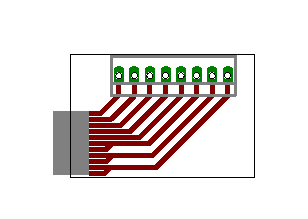
\includegraphics[width=0.5\textwidth]{figures/expansion_board.pdf}
	\caption{Left leg extension PCB schematic}
	\label{fig:pcb1}
\end{figure}

% subsubsection extension_pcbs (end)


% subsection electric_actuators (end)
%!TEX root = ../../../../report.tex

\subsection{Sensory feedback} % (fold)
\label{sub:sensory_feedback}
As stated in the initial description of the project in \ref{sec:overall_description}, the first prototype of Rubi has been designed to provide the necessary capabilities to be controlled by an existing neural controller developed in \cite{dacbot1} and already tested in the DACbot robot.
The cited control algorithm requires as inputs the angular positions of all the joints in can actuate, besides ground contact signals from the feet for its reflex-based controller part.
All the documentation regarding the handling of the sensor readings software-wise is to be found in section \ref{sec:software}.


\subsubsection{Joint position information} % (fold)
\label{ssub:joint_position_feedback}
To provide the physical readings of the angular positions of the joints, the built-in hall sensors in the motors are utilized. 
Three wires transmit the hall effect sensors signals to the motor board for each joint, where they are written in the internal register and transferred to the main processor for its posterior treatment.
% subsubsection joint_position_feedback (end)

\subsubsection{Ground contact signal} % (fold)
\label{ssub:ground_contact_feedback}
One contact switch model Omron D2F-01F-T has been placed on the edge of the sole of each foot, under the heel in order to detect when the feet are standing on the ground. 
Their wiring has been extended to the main processor board, but the necessary pull-up resistors have not been implemented since the input pins on the processor could not be set up.
The necessary mapping between the processor's GPIOS handlers and the physical pins on the board could not be found.
Therefore this last step is left as further work.
Alternatives to the use of the main board pins are discussed in chapter \ref{cha:discussion}, in case they cannot be used.
% subsubsection ground_contact_feedback (end)

% subsection sensory_feedback (end)

% section electronics (end)
%!TEX root = ../../../report.tex
\section{Mechanics} % (fold)
\label{sec:mechanics}

%!TEX root = ../../../../report.tex
\subsection{Pulleys and belts} % (fold)
\label{sub:pulleys_and_belts}
The section \ref{sec:joints} is dedicated to analyze and define what kind of motors and trasmision system is going to be used for each joint.
In the case of the knee and the ankle, the combination \textit{motor + gearbox + belt and pulleys} is chosen due to the preference of having the active actuator in the highest part of the link with the withdrawal of transfer the movement the the lowest.
This system has been design along with the torsional springs disussed in the section \ref{sub:compliance} where the rotation from the motor must feed the rotation of a serial rotational spring.
This implies the design of a system in which pulley and spring holder must be gathered.
The design of the pulley itself though, has been studied in terms of two factors: \textit{precision and backlash reduction} and \textit{integration with the serial rotational spring}.

\subsubsection{Precision and backlash reduction} % (fold)
\label{ssub:precision_and_backlash_reduction}
The goal of this design was to optimize the pulley to get a lack of backlash.
Despite the platform is going to be used mainly for self-learning controllers (e.g. based on neuronal networks) and then the mechanical optimization is not a priority, the reduction of mechanical uncertainty is always good.

After analyze all the current market several non-backlash solutions are found.
Stands out the Gates GT3 Synchronous Belts \footnote{http://www.gates.com/products/industrial/industrial-belts/synchronous-belts/powergrip-gt3-belts} that is assured to be suitable for the presented application.
The withdrawals of this design are the lack of time for ordering such parts and the increase in the final price of the product. 
However there is another important factor, the integration that must be done with the serial rotational spring.
% subsubsection precision_and_backlash_reduction (end)

\subsubsection{Integration with the serial rotational spring} % (fold)
\label{ssub:integration_with_the_serial_rotational}
Another solution is to design the pulley itself which would let to have a complete control of the design and manufacturability giving the possibility of integrate in a unique part design, the pulley for the transmission system and the spring holder.

At first, the GT3 design from Gates was intended to be designed.
However, its design is described in U.S. Patent Number 4,515,577, which doesn't allow its use.
Thus, the belts have been designed following the ISO 13050:2014 \cite{ISO13050} following the type T due to its focus in efficiency and reduction of backlash.
It is also appropriate for precision movements, high torques and low speeds, as our requirements.

The physical properties of the pulleys as the number of teeth, width, etc... have been chosen based on the ISO 5295:1987 \cite{ISO5295} and in sake of manufacturability.
As decided before, the pulley will belong to a part that will also have the task of holding the rotational serial spring.
This implies that the part will be designed to be 3D printed and thus, the criteria of design oriented to manufacturability must be applied.

Based on both ISO norms cited before and after some iterations based on experimental tests the pulley T2,5 of 19 teeth gave the expected behavior.
Both pulleys are the same so no reduction is given from the motor shaft to he other.
In the figure \ref{fig:motor_pulley}, a detail of the designed pulleys can be seen.
% subsubsection integration_with_the_serial_rotational (end)

% subsection pulleys_and_belts (end)
%!TEX root = ../../../../report.tex
\subsection{Gears} % (fold)
\label{sub:gears}

% subsection gears (end)
%!TEX root = ../../../../report.tex
\subsection{Impact force} % (fold)
\label{sub:impact_force}
In order to calculate the physical dimensions of some of the components, a bounding conditions have to be defined.
The presented case shows a peak of energy when landing after being jumped a estimated height.
This energy in then transmitted from the first contact point, the footprint, to the rest of the system, causing efforts that must be absorbed.
The components of the system must receive that energy under a controlled behavior -this is elastic deformations- assuring a longer life cycle of the legs.

Thus, some input parameters to calculate the impact force are assumed.
From this force will be sized all the consecutive components in the deformation chain.
Despite the deformation is of the whole system, the security coefficient assumed in here is going to be the calculation of all the components for that maximum force.

From the formula of the mechanical energy:
\begin{equation}
  E_{mechanical} = m g \Delta h + \frac{1}{2} m v^{2}
\end{equation}

The kinetic energy is negligible and only the energy form falling a certain height is supposed.
This energy is then translated into force by supposing a deformation of the whole body:
\begin{equation}
\label{eq:impact_force}
  F_{impact} = \frac{m g \Delta h}{t_{impact\_displacement}}
\end{equation}

The equation \ref{eq:impact_force} gives the force for sizing all the components.
Based on the input parameters defined in the appendix \ref{app:profile_selection} which are:
\begin{table}
\begin{center}
\begin{tabular}{c | c}
  Parameter & Value \\
  \hline
  Total mass [kg] & 1.5 \\
  Jumping height [m] & 0.1 \\
  Impact displacement [m] & 0.005
\end{tabular}
\caption{Input parameters for calculating the impact force}
\label{tab:input_parameter_impact_force}
\end{center}
\end{table}

The impact force is then:
\begin{equation}
  F_{impact} = \frac{m g \Delta h}{d_{impact\_displacement}} = 294.40 N 
\end{equation}
% subsection impact_force (end)
%!TEX root = ../../../../report.tex
\subsection{Limb profile} % (fold)
\label{sub:limb_profile}
Based on the requirements of weight and its distribution defined in the analysis of the joints \ref{sec:joints}, the links have been decided to have in the upper extreme the actuators. 
This leads to use a transmission system, such as belt and pulleys, which leaves for the rest of link a structural function that can also adopt the task of wiring placement.
Thus, a light weight section that satisfy the conditions of deformation and stress maximum will be chosen.
Carbon fiber is an ideal material to achieve this conditions of weight and stress so an quantitative analysis has been made calculating the optimal solution and then rounding it for all the possible profiles offered by the given provider.
The provider was chosen due to the previous experiences that the Mærsk Mc-Kinney Møller Institute had with carbon fiber orders.

The section profile offered \footnote{http://www.easycomposites.co.uk/\#!/cured-carbon-fibre-products/} are: \textit{Rod}, \textit{Tube}, \textit{Box}. The \textit{Stripe} and the \textit{Angle} are discarded due to its asymmetrical geometry that will will lead to less predictable scenarios.
The study case is show in the figure \ref{fig:impact_decomposition}, where the impact force can be decomposed in a pure bending effort and a pure compression.
Due to the resistance of the carbon fiber in pure compression is bigger than in bending, only this last case has been studied.
This studies should not completly follow the behaviour in real life due to the carbon fiber is not an isomorphic material.
However, the high security factor taken into account is expected to overcome this assumption.

\begin{figure}[ht!]
  \centering
  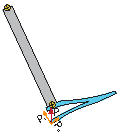
\includegraphics[width=.3\textwidth]{figures/impact_decomposition.pdf}
  \caption{Impact force decomposed}
  \label{fig:impact_decomposition}
\end{figure}

\subsubsection{Profile study} % (fold)
\label{ssub:profile_study}
  The bending effort causes two sort of problems: (1) the possible break in the supporting point and (2) the deformation suffered by the beam.
  The break will occur when the tensions created will be over the ultimate tension in compression or tension of the selected material.
  This comes defined in the equation \ref{eq:tension} for symmetric sections and when an only torque is being applied.
  \begin{equation}
  \label{eq:tension}
    \sigma _{compression} = \sigma _{tension} = \frac{M h_{CG}}{I_x}
  \end{equation}

  Meanwhile the deformation in the extreme can be calculated with the equation \ref{eq:deformation} if the case is simplified to the occurred in the figure \ref{fig:impact_decomposition}.
  This is, when the legs is completely stretched, what will cause the biggest stresses.

  \begin{figure}[ht!]
    \centering
    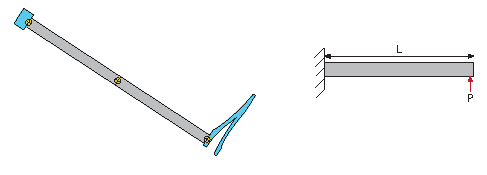
\includegraphics[width=\textwidth]{figures/bending_case.pdf}
    \caption{Simplified representation of the bending case}
    \label{fig:bending case}
  \end{figure}

  \begin{equation}
  \label{eq:deformation}
    y_L = \frac{P z^2}{6EI}(3L-z) = \frac{P L^2}{6EI}(2L) = \frac{P L^2}{3EI}
  \end{equation}


  For the selected profiles the equations that define the compression $\sigma _{compression}$ and tension efforts $\sigma _{tension}$, along with the deformation in the direcction of the applied force $y_L$ are shown, being:

  \begin{enumerate}
    \item $h_{CG}$: height of the center of gravity of the semi-half section from the geometrical center of the section.

    \item $E$: Elastic module.
  \end{enumerate}


  \noindent\begin{minipage}{0.2\textwidth}% adapt widths of minipages to your needs
      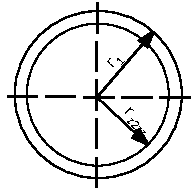
\includegraphics[width=\linewidth]{figures/profile_cylinder.pdf}
  \end{minipage}%
  \hfill%
  \begin{minipage}{0.8\textwidth}
    \begin{equation}
      \begin{aligned}
      \sigma _{compression} = \sigma _{tension} &= \frac{M h_{CG}}{I_x} = \frac{4 r_2}{\pi(r_2 ^4 - r_1 ^4)} M \\
      y_L &= \frac{P L^2}{3EI} = \frac{4 P L^2}{3 E \pi(r_2 ^4 - r_1 ^4)}\\
      h_{CG} &= r_2 \\
      I_x = I_y &= \frac{\pi}{4} (r_2 ^4 - r_1 ^4)
      \end{aligned}
    \end{equation}
  \end{minipage}

  \noindent\begin{minipage}{0.2\textwidth}% adapt widths of minipages to your needs
      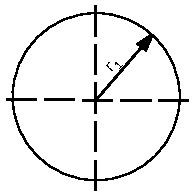
\includegraphics[width=\linewidth]{figures/profile_tube.pdf}
  \end{minipage}%
  \hfill%
  \begin{minipage}{0.8\textwidth}
    \begin{equation}
    \begin{aligned}
      \sigma _{compression} = \sigma _{tension} &= \frac{M h_{CG}}{I_x} = \frac{4}{\pi r_1 ^3} M\\
      y_L &= \frac{P L^2}{3EI} = \frac{4 P L^2}{3 E \pi r_1 ^4}\\
      h_{CG} &= r_1 \\
      I_x = I_y &= \frac{\pi r_1 ^4}{4}
      \end{aligned}
    \end{equation}
  \end{minipage}

  \noindent\begin{minipage}{0.2\textwidth}% adapt widths of minipages to your needs
      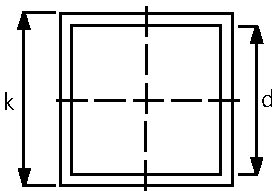
\includegraphics[width=\linewidth]{figures/profile_squared.pdf}
  \end{minipage}%
  \hfill%
  \begin{minipage}{0.8\textwidth}
    \begin{equation}
    \begin{aligned}
      \sigma _{compression} = \sigma _{tension} &= \frac{M h_{CG}}{I_x} = \frac{6 d}{(d^4 - k^4)}\\
      h_{CG} &= \frac{d}{2} \\
      y_L &= \frac{P L^2}{3EI} = \frac{4 P L^2}{E (d^4 - k^4)}\\
      I_x = I_y &= \frac{1}{12} (d^4 - k^4)
      \end{aligned}
    \end{equation}
  \end{minipage}
% subsubsection profile_study (end)

\subsubsection{Torque calculation} % (fold)
\label{ssub:torque_calculation}
  For both cases, the profile of the lower limb and the upper, the torque generated by the impact force determined in the section \ref{sub:impact_force}, is calculated.
  This torque is different in the lower and the upper limb due to the upper limb takes the distance from the foot to the hip while the other one is only from the foot to the knee:
  \begin{equation}
  \begin{aligned}
     M_{lower\ limb} = F \cdot d = 294.4 \cdot 0.2126 = 62.57 Nm\\
     M_{upper\ limb} = F \cdot d = 294.4 \cdot (0.2126 + 0.2622) = 139.73 Nm
  \end{aligned}
  \end{equation}
% subsubsection torque_calculation (end)

\subsubsection{Final limb parameters} % (fold)
\label{ssub:final_limb_parameters}
Following the criteria from the sections \ref{sec:dimensions} and \ref{sec:physical_properties} of size and materials, the presented formulas and the have been applied to all the profiles of the provider.
An iterative processes based on the outputs of the mathematical model \ref{cha:mathematical_model} has given a result the limb lengths shown in the table \ref{tab:limb_lengths}.

\begin{table}[ht!]
\centering
\caption{Final limb lengths}
\label{tab:limb_lengths}
\begin{tabular}{r|l}
  \textbf{Limb} & \textbf{Length [m]} \\ \hline
  Foot & 0.095 \\ \hline
  Lower limb & 0.212 \\ \hline
  Upper limb & 0.262    
\end{tabular}
\end{table}

\todo{Add hip and foot width with small explanation}

Then, the profiles have been analyzed calculating the torque from \ref{ssub:torque_calculation} and then applying the section \ref{ssub:profile_study} for each iteration.
The calculations of the last iteration are shown in the appendix \ref{app:profile_selection}.
These results have been then approved or discarded based on a \textit{maximum deformation} and \textit{ultimate tension} requirements, and are shown in the table \ref{tab:profile_selection}

\begin{table}[ht!]
\centering
\caption{Profile selection for each limb}
\label{tab:profile_selection}
\begin{tabular}{c|c|c}
  \textbf{Limb} & \textbf{Section} & \textbf{Dimensions} \\ \hline
  Lower limb & Tube & 20 mm and 1 mm thickness \\ \hline
  Upper limb & Tube & 20 mm and 1 mm thickness 
\end{tabular}
\end{table}

% subsubsection profile_selection (end)



% subsection limb_profile (end) 
%!TEX root = ../../../../report.tex

\subsection{Bearings} % (fold)
\label{sub:bearings}
In the section \ref{sub:impact_force} the force for sizing the bearings of the knee and the ankle was calculated.
The bearing elected would be such that allows dynamic loads of more than the impact force while keeping as small as possible to reduce the added weight to the robot.
On the other hand, the internal diameter comes defined by the rod diameter calculated in the section \ref{sub:rods}.

An estimation of nominal life of the bearing can be done from the Dynamic Load Rating (C), the Dynamic Equivalent Load (P) and the Life Rime Coefficient for a Ball Bearing (p) (being p=3 for balls bearings).
The equation \ref{eq:service_life_bearing}, shows the nominal life of a ball bearing that can be used in order to calculate the nominal life for a specific application.
It is also worth to mention that the Dynamic Equivalent Load (P) is divided by the number of bearings in which the force is spread.
\begin{equation}
  \label{eq:service_life_bearing}
  L_{10} = \frac{10^{6}}{60 n} \left(\frac{C}{P}\right)^{p}
\end{equation}

The term $L$ is the service life of a bearing (in number of hours or rpm), in normal conditions of speed and load, in which the bearing is working until fail by fatigue. 
Whilst $L_{10}$ is based in a stadistical model that is defined as the 90\% of the bearing of the same type will withstand those loads for a longer time.
% subsection bearings (end)
%!TEX root = ../../../../report.tex
\subsection{Rods} % (fold)
\label{sub:rods}
As explained in section \ref{sub:bearings}, was decided to have two bearings per link (which gives four per joint) and a rod going through them.
This rod is then also used, in the case of the knee and the ankle, as a support for the pulleys that transmit the power from the pulley to the next link.

Three mechanical efforts bound its design:
\begin{enumerate}
  \item \textbf{Shear strenth}: in the case of the shear produced when an impact occurs and the rod of one link moves in the opposite direcction than its relative in the consecutive link.
  \item \textbf{Resistance to beding}: due to the bending effort that the tension of the belt is constantly applying in the rod of the  knee and the ankle.
  \item \textbf{Torsion}: due to the pulley in the knee and the ankle. 
  This effort is negligible because zero-friction bearings are supposed.
\end{enumerate}

  \subsubsection{Shear analysis} % (fold)
  \label{ssub:shear_analysis}
  The maximum shear stress is found in the diameter of the cylinder (y=0) and is:
  
  \noindent\begin{minipage}{0.2\textwidth}% adapt widths of minipages to your needs
  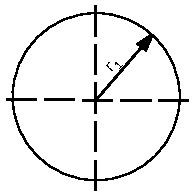
\includegraphics[width=\linewidth]{figures/profile_tube.pdf}
  \end{minipage}%
  \hfill%
  \begin{minipage}{0.8\textwidth}
    \begin{equation}
    \begin{aligned}
      \gamma_{yz} &= \frac{Q_y M_{x}^A*}{b(y) I_x} = \frac{Q}{r^2}\\
      M_{x}^{A_{y=0}} &= \frac{\pi r_1^2}{2} \\
      b(y=0) &= 2 r_1 \\
      I_x &= \frac{\pi r_1^4}{4}
      \end{aligned}
    \end{equation}
  \end{minipage}
  Given a tangent force Q, the shear stress can be calculated.
  If this is over the ultimate strength, the cylinder will break.
  % subsubsection shear_analysis (end)

  \subsubsection{Bending} % (fold)
  \label{ssub:bending}
  The beding analisys follows the one carried out in the section \ref{ssub:profile_study} for a cylinder.
  The equivalent force in this case is given by the tension of the belts, mainly the initial (thought there are other tensions that appear when the belts moves).
  Due to feasibility reasons an the lack of measurements units, some experimental tests trying differnt tensions and axis where carried out giving good results with a 3 mm rod or more.
  % subsubsection bending (end)

  \subsubsection{Sizing} % (fold)
  \label{ssub:sizing}
  The studies above have been tested for different diameters of rod starting from the smallest size given by the provider and increasing until both conditions are satisfied, due to the requirements of low weight.
  In case of using steel as material, the ultimate strength is supposed to be 250 MPa \footnote{https://en.wikipedia.org/wiki/A36\_steel}.
  And for the case of a rod of 3 mm of diameter, both stresses are under the restrictions.
  Thus, 3 mm rods are going to be used.
  % subsubsection sizing (end)
% section rods (end)
%!TEX root = ../../../../report.tex

\subsection{Finite Element Method (FEM)} % (fold)
\label{sub:finite_element_method}

% subsection finite_element_method (end)
%!TEX root = ../../../../report.tex
\subsection{Computer-Aided Design (CAD)} % (fold)
\label{sub:computer_aided_design}

\begin{figure}[ht!]
    \centering
    \begin{subfigure}[b]{0.49\textwidth}
        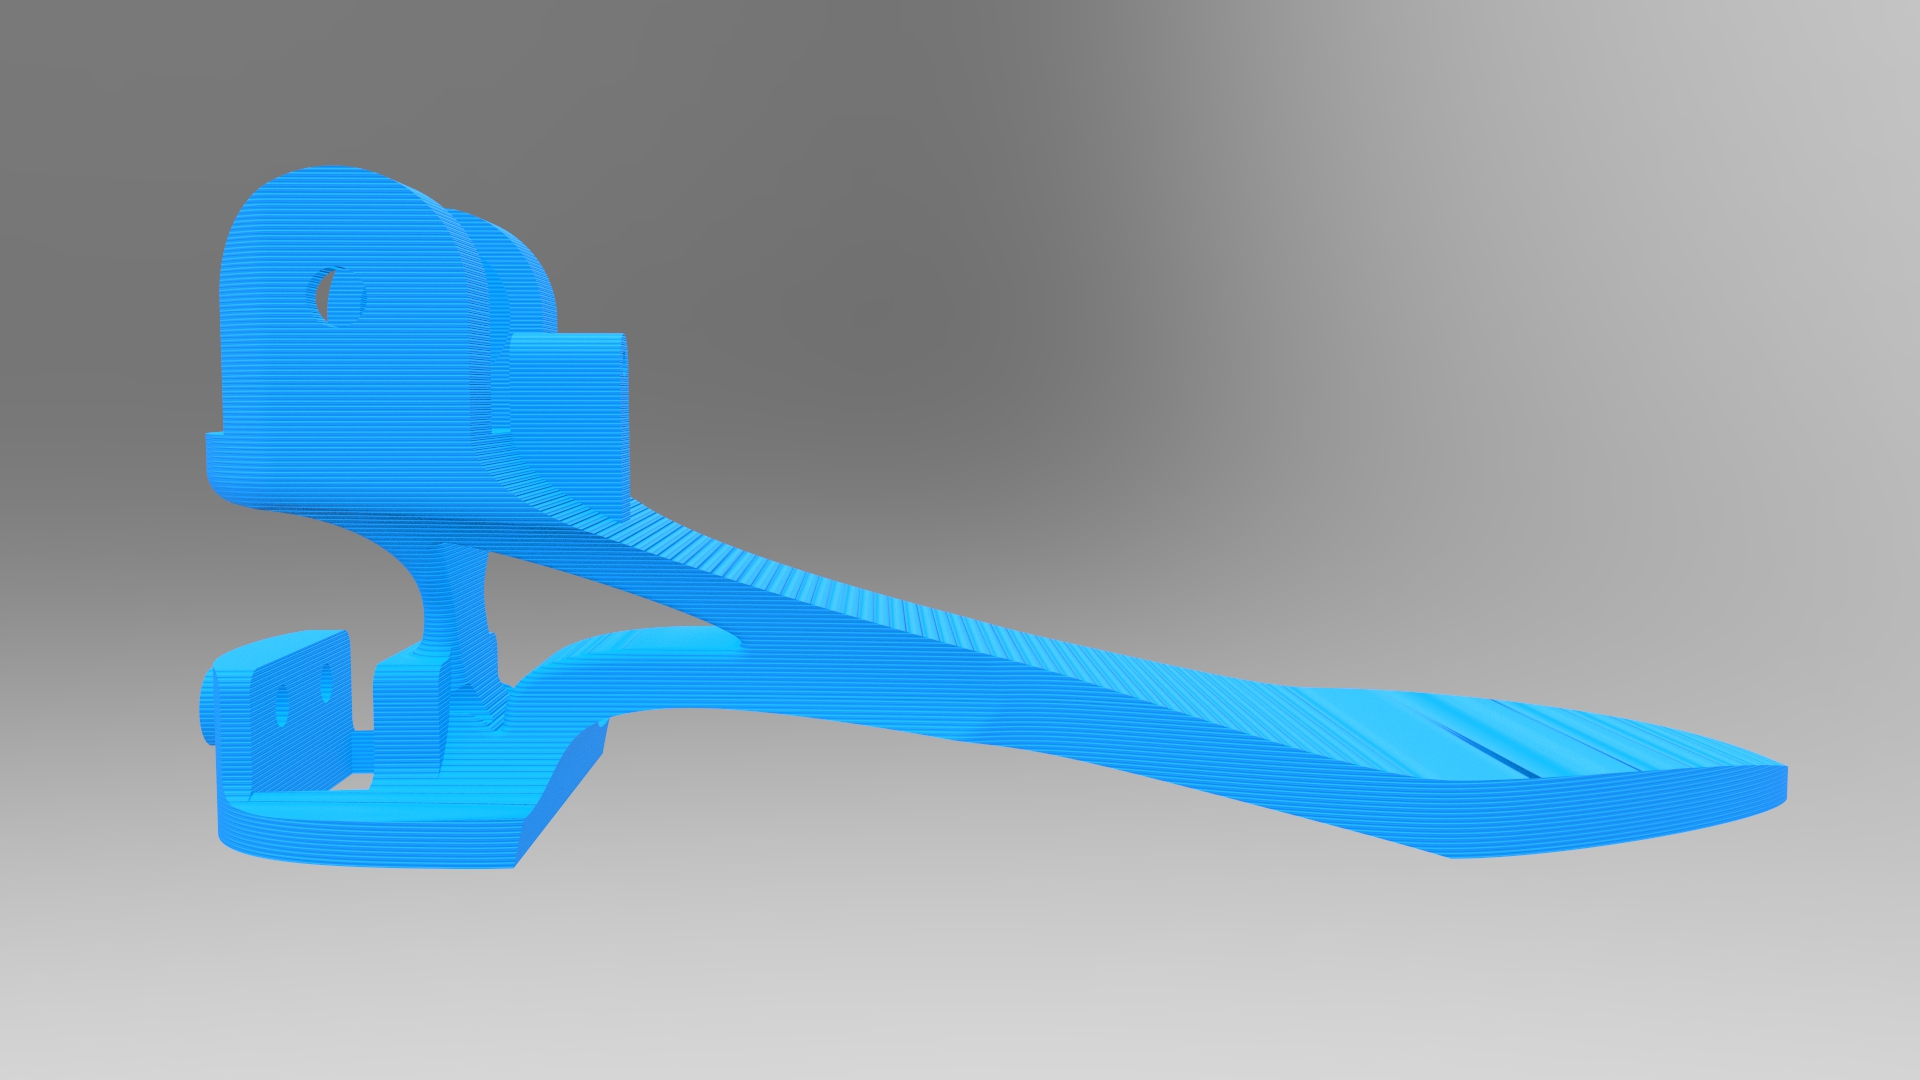
\includegraphics[width=\textwidth]{figures/legs_foot.jpg}
        \caption{Left foot}
        \label{fig:left_foot}
    \end{subfigure}
    \begin{subfigure}[b]{0.49\textwidth}
        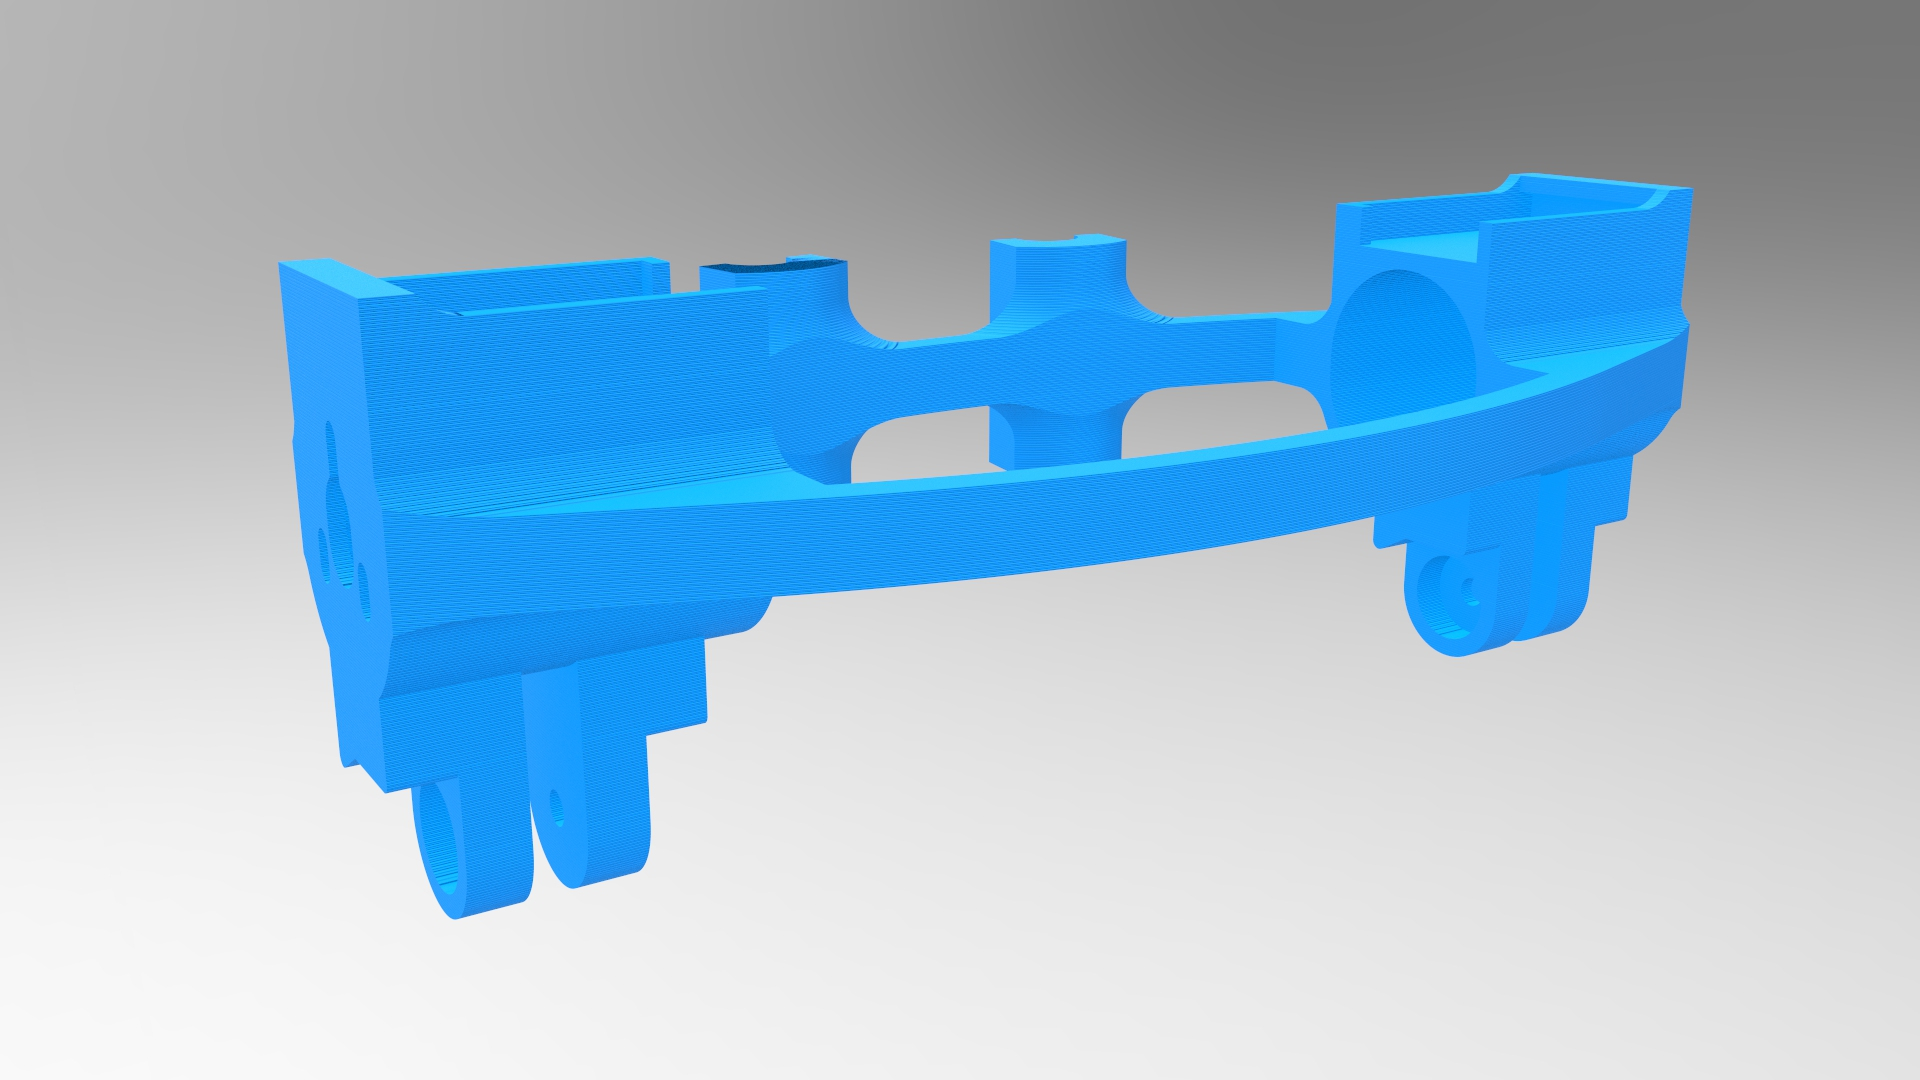
\includegraphics[width=\textwidth]{figures/legs_hip.jpg}
        \caption{Hip}
        \label{fig:hip}
    \end{subfigure}

    \begin{subfigure}[b]{0.49\textwidth}
        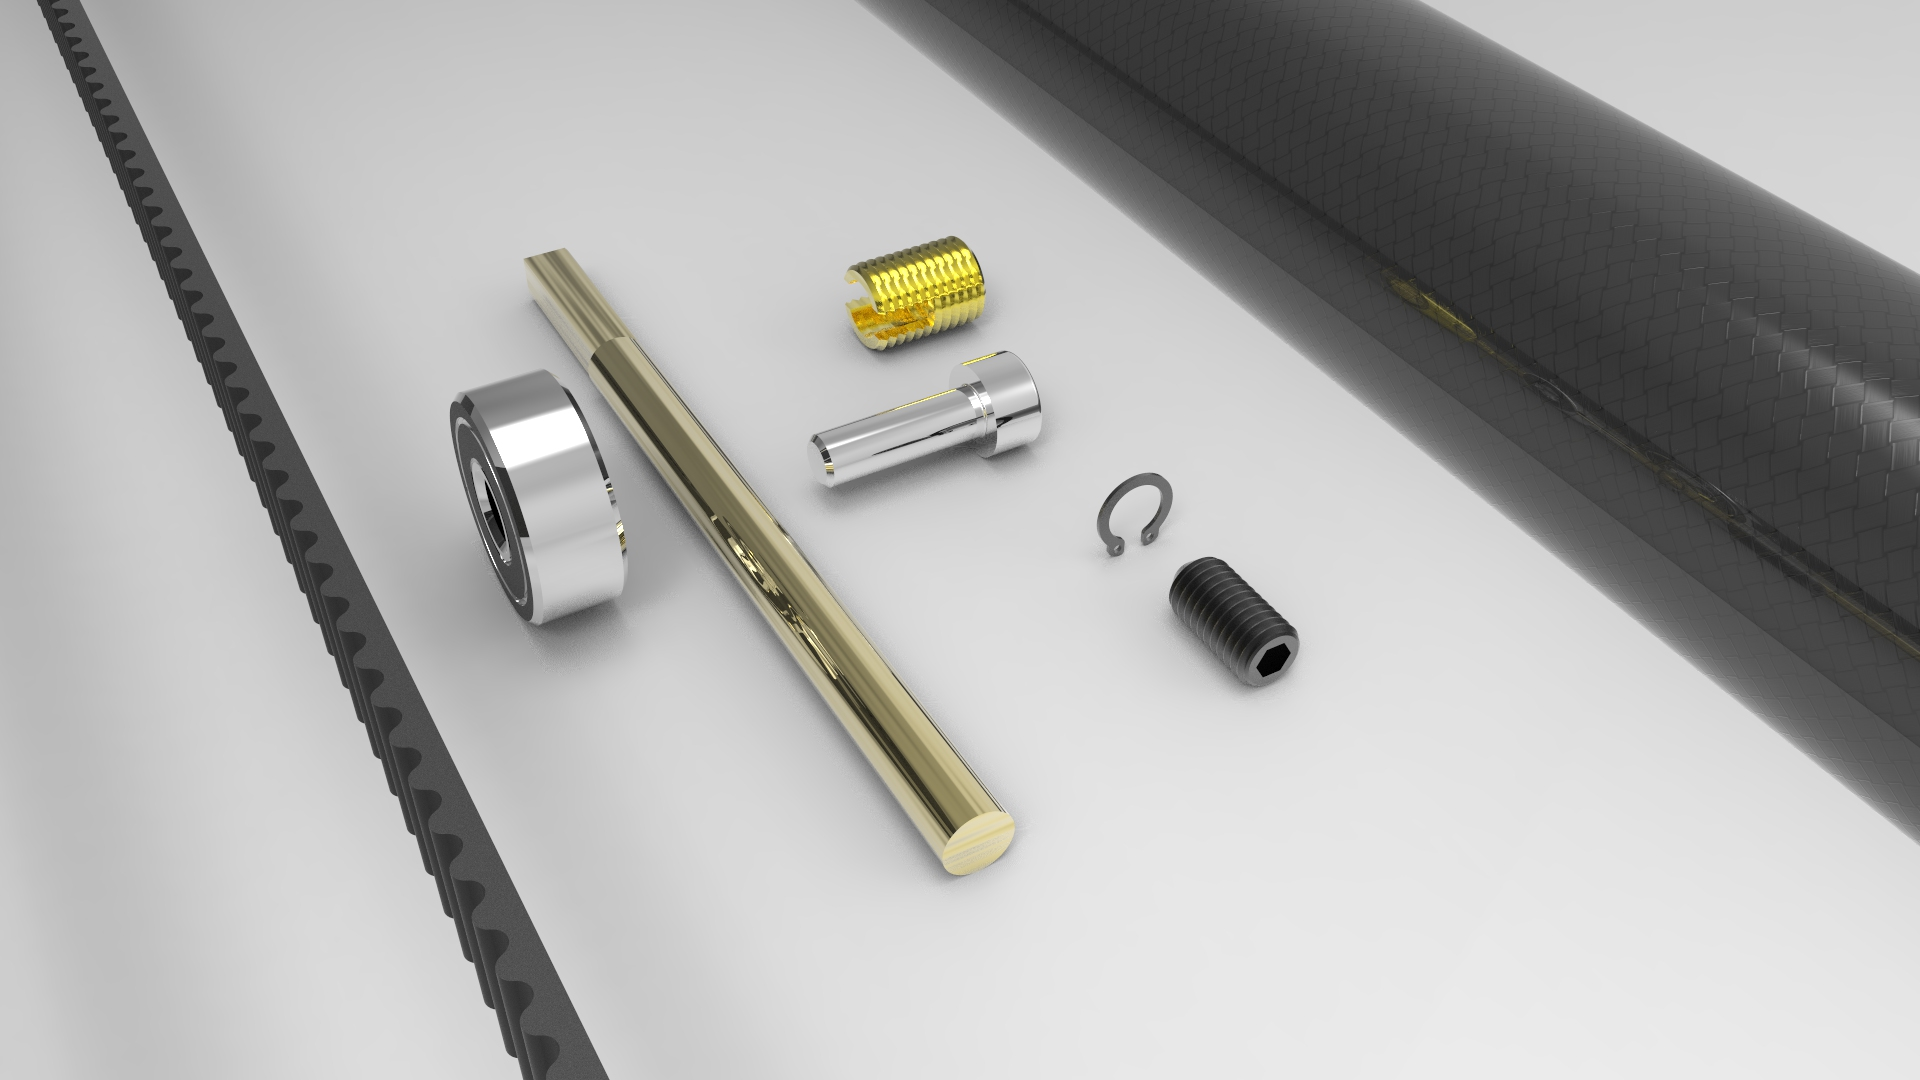
\includegraphics[width=\textwidth]{figures/legs_parts.jpg}
        \caption{Additional designed parts}
        \label{fig:mouse}
    \end{subfigure}
    \begin{subfigure}[b]{0.49\textwidth}
        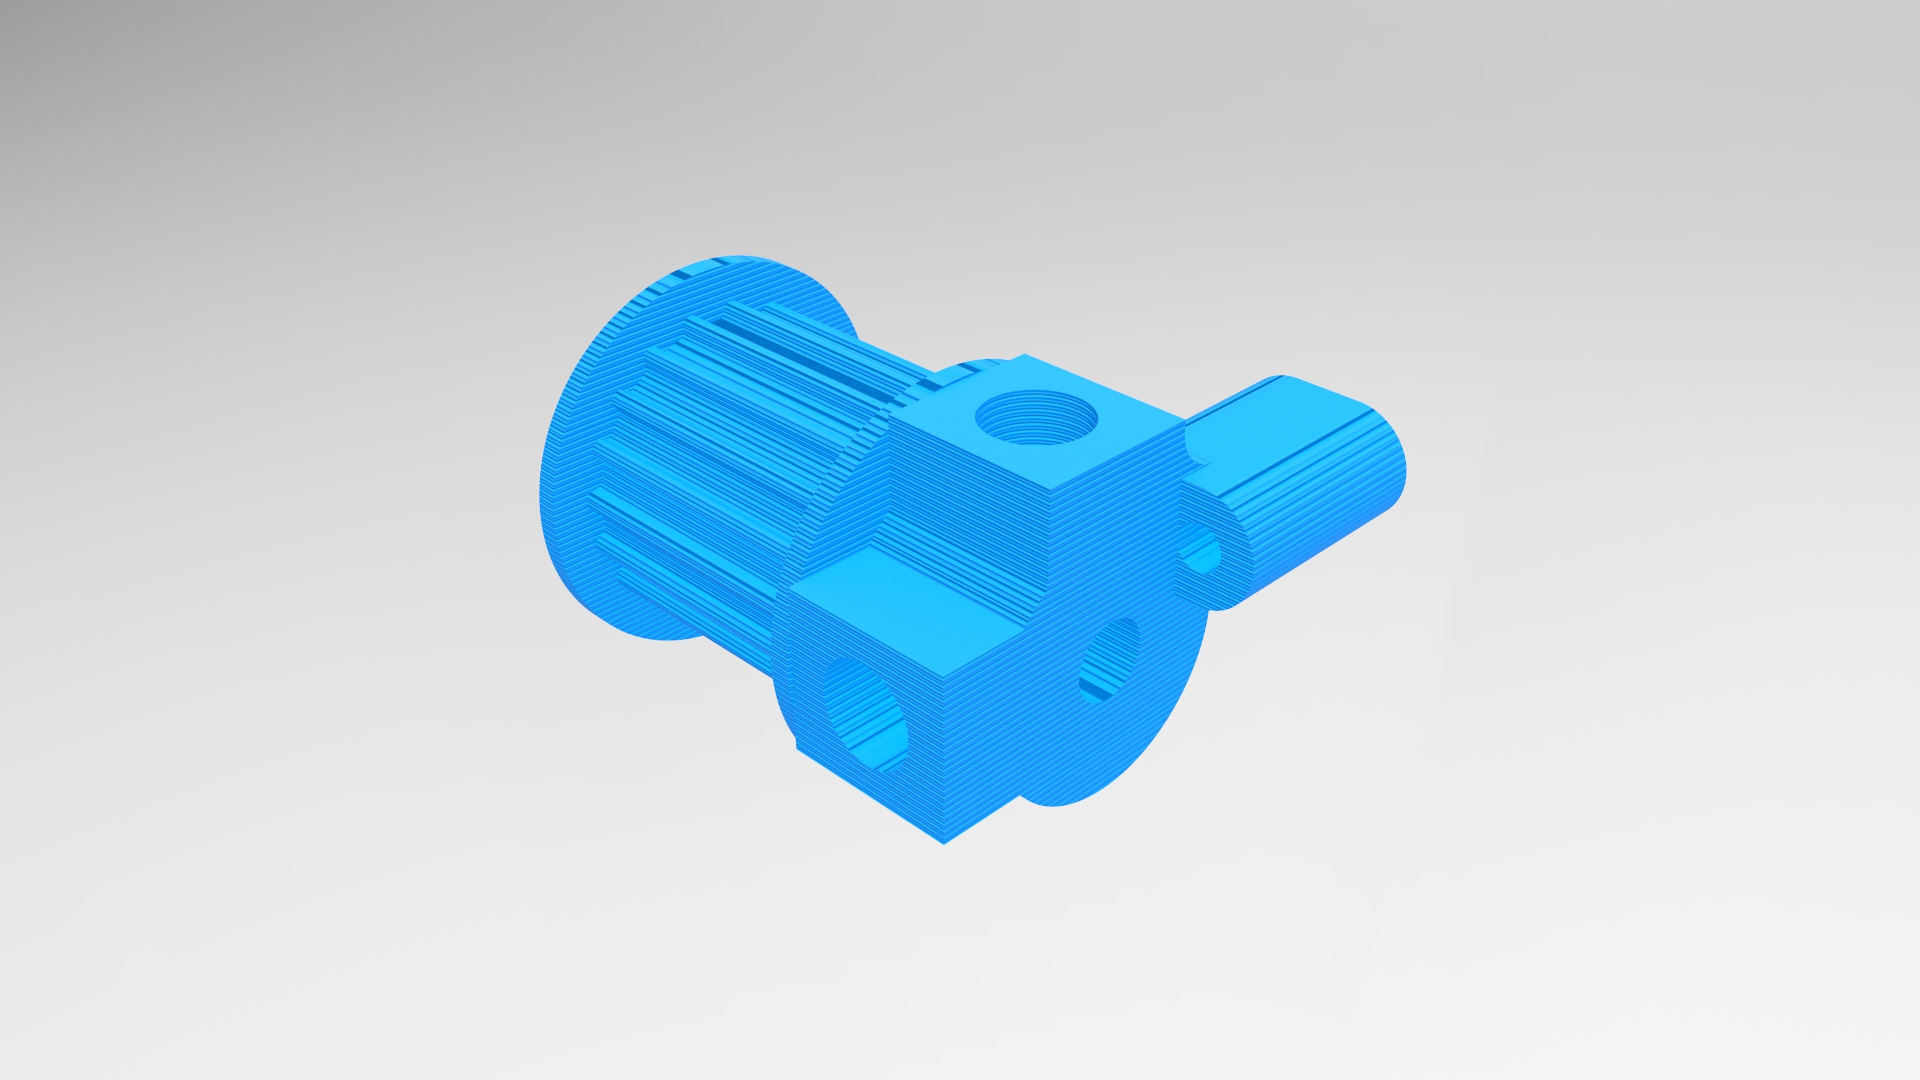
\includegraphics[width=\textwidth]{figures/legs_pulley.jpg}
        \caption{Left ankle serial spring pulley}
        \label{fig:serial_spring_pulley}
    \end{subfigure}

    \begin{subfigure}[b]{0.49\textwidth}
        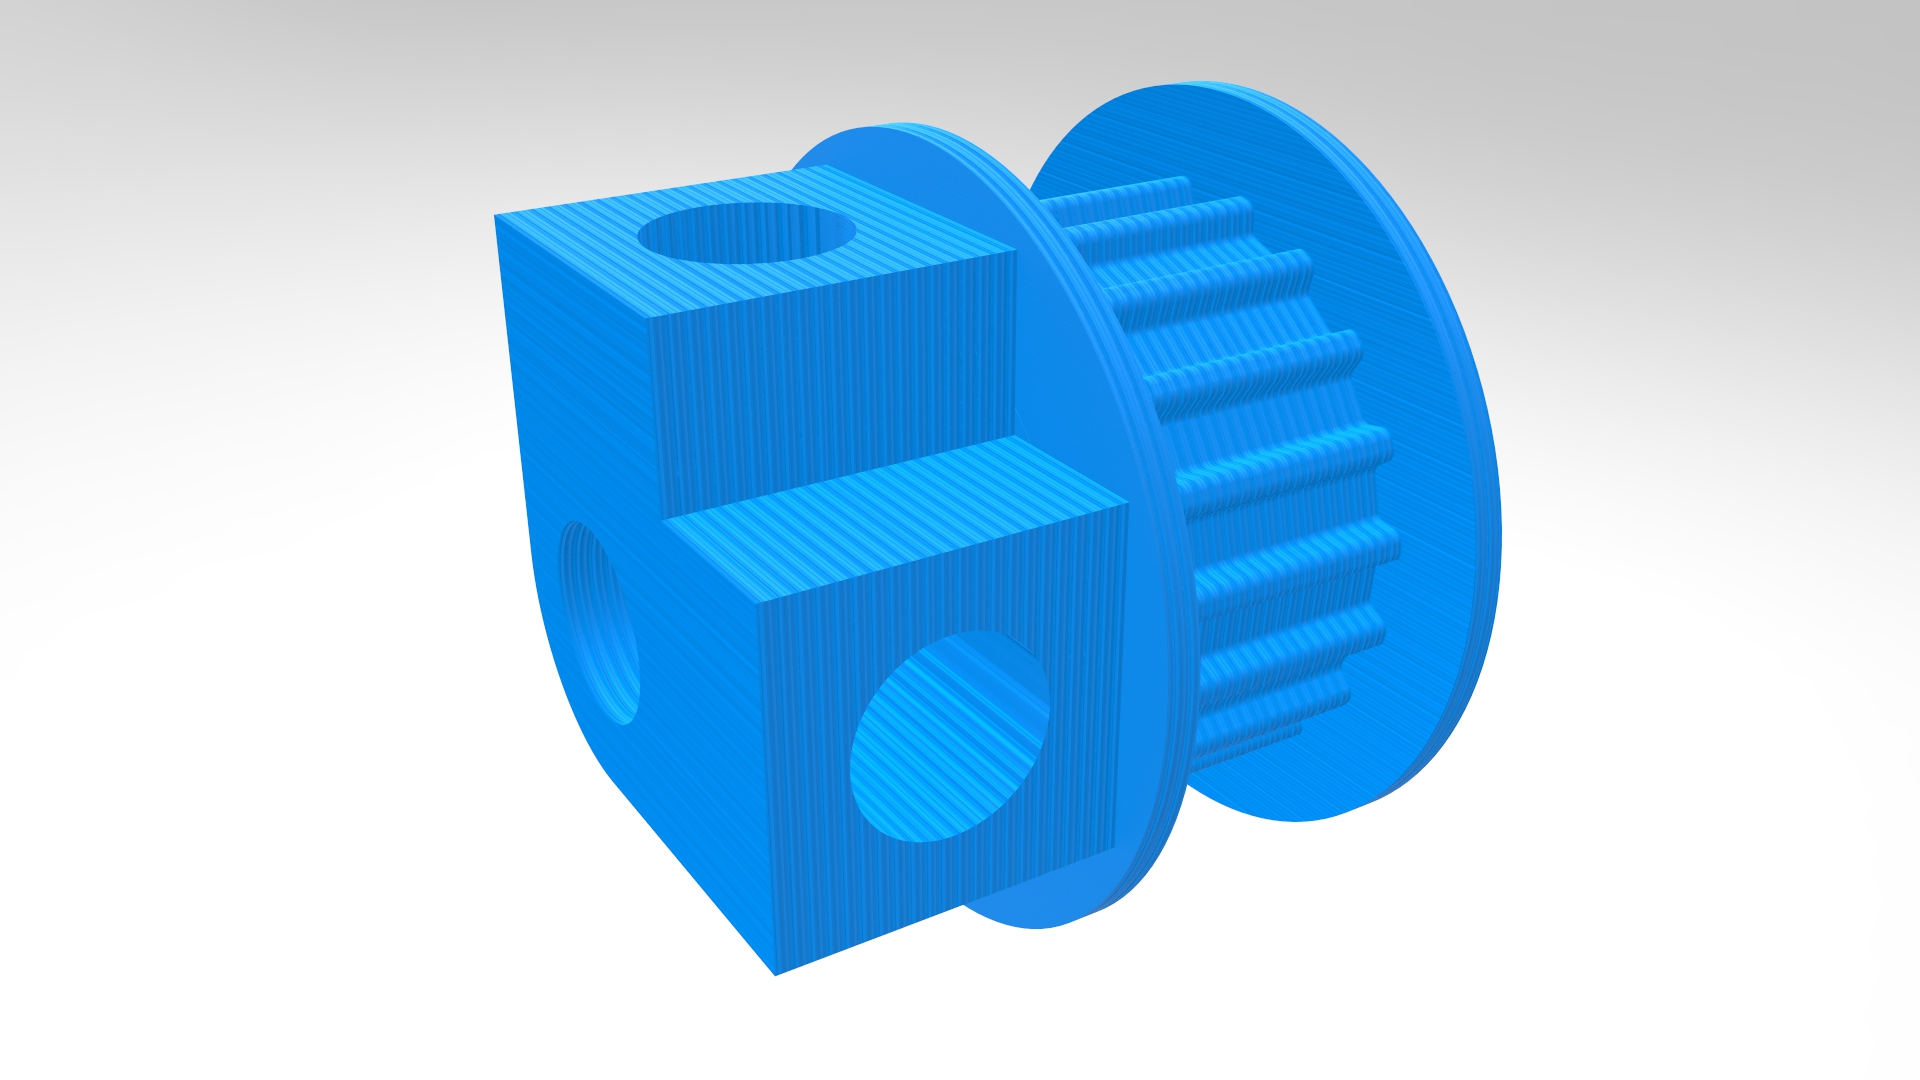
\includegraphics[width=\textwidth]{figures/legs_pulley_motor.jpg}
        \caption{Motor pulley}
        \label{fig:motor_pulley}
    \end{subfigure}
    \begin{subfigure}[b]{0.49\textwidth}
        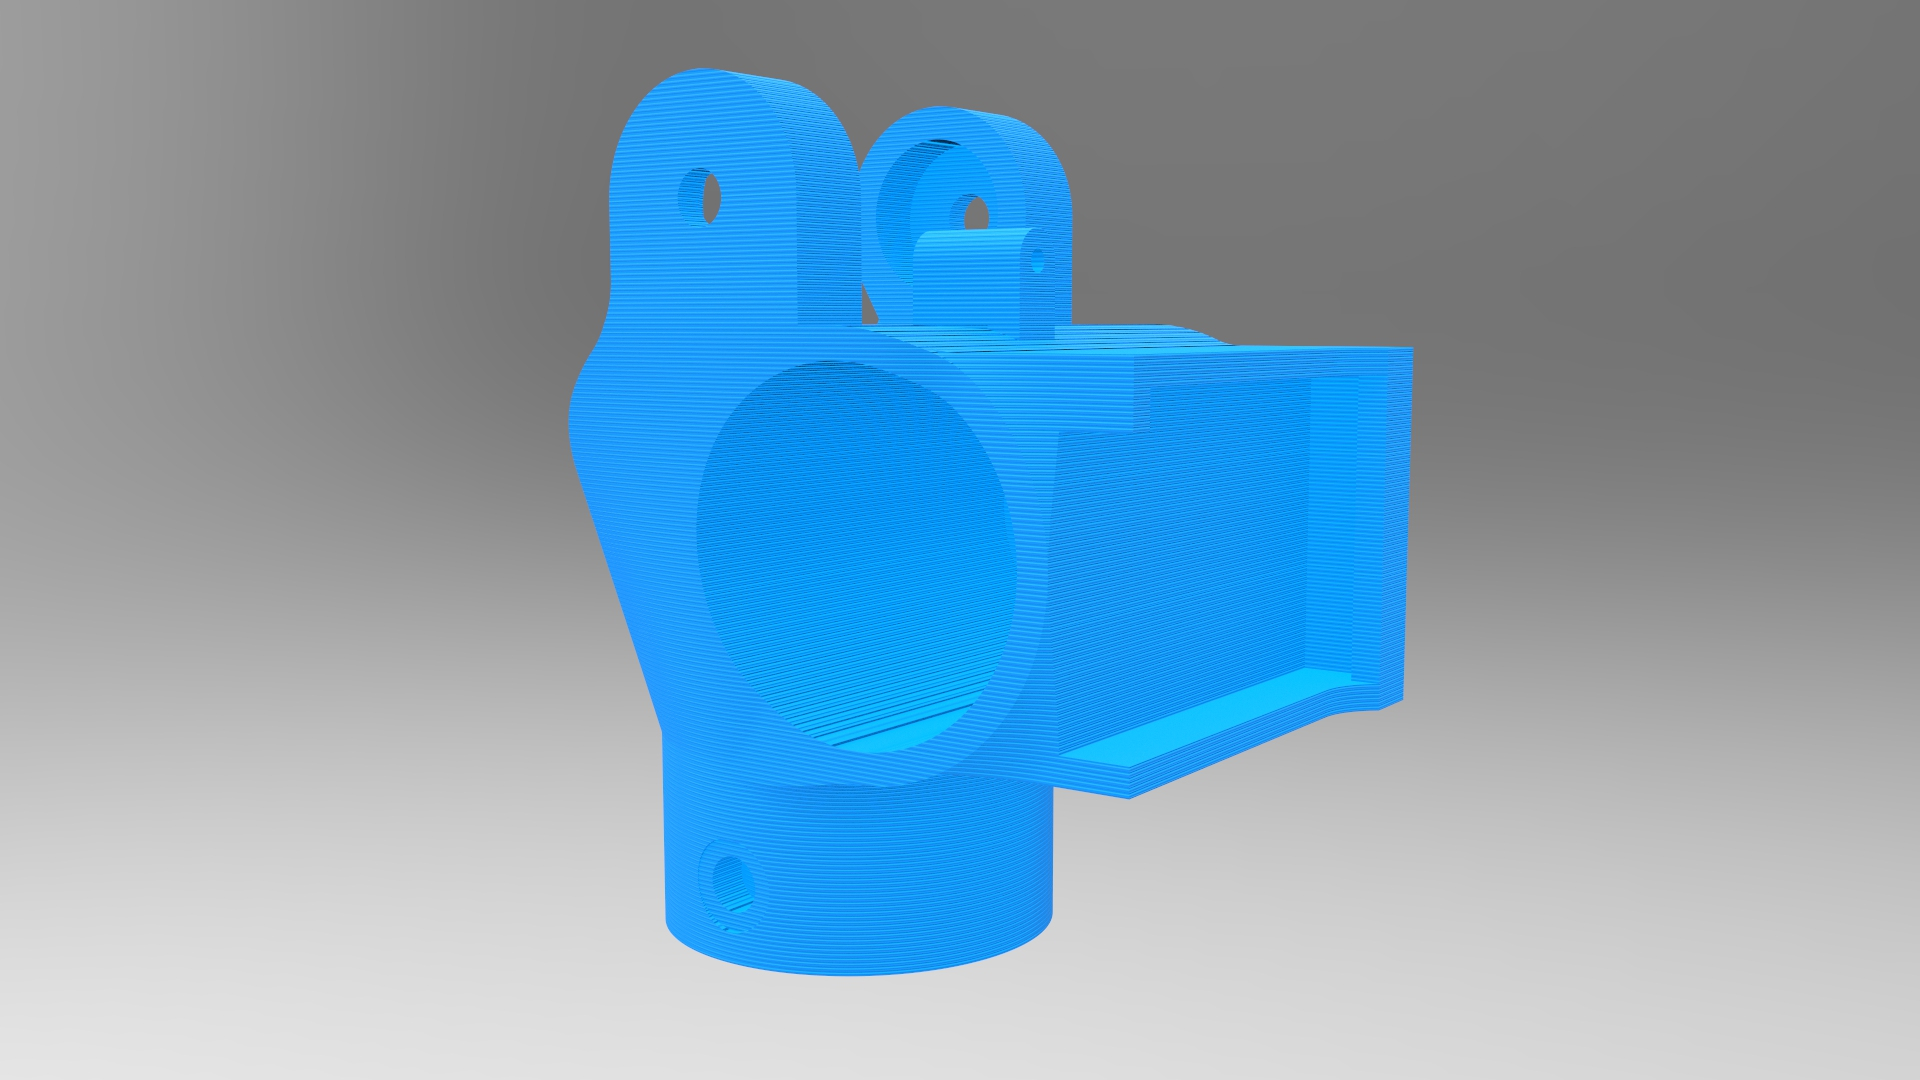
\includegraphics[width=\textwidth]{figures/legs_knee_lower.jpg}
        \caption{Left lower knee}
        \label{fig:lower_knee}
    \end{subfigure}

    \begin{subfigure}[b]{0.49\textwidth}
        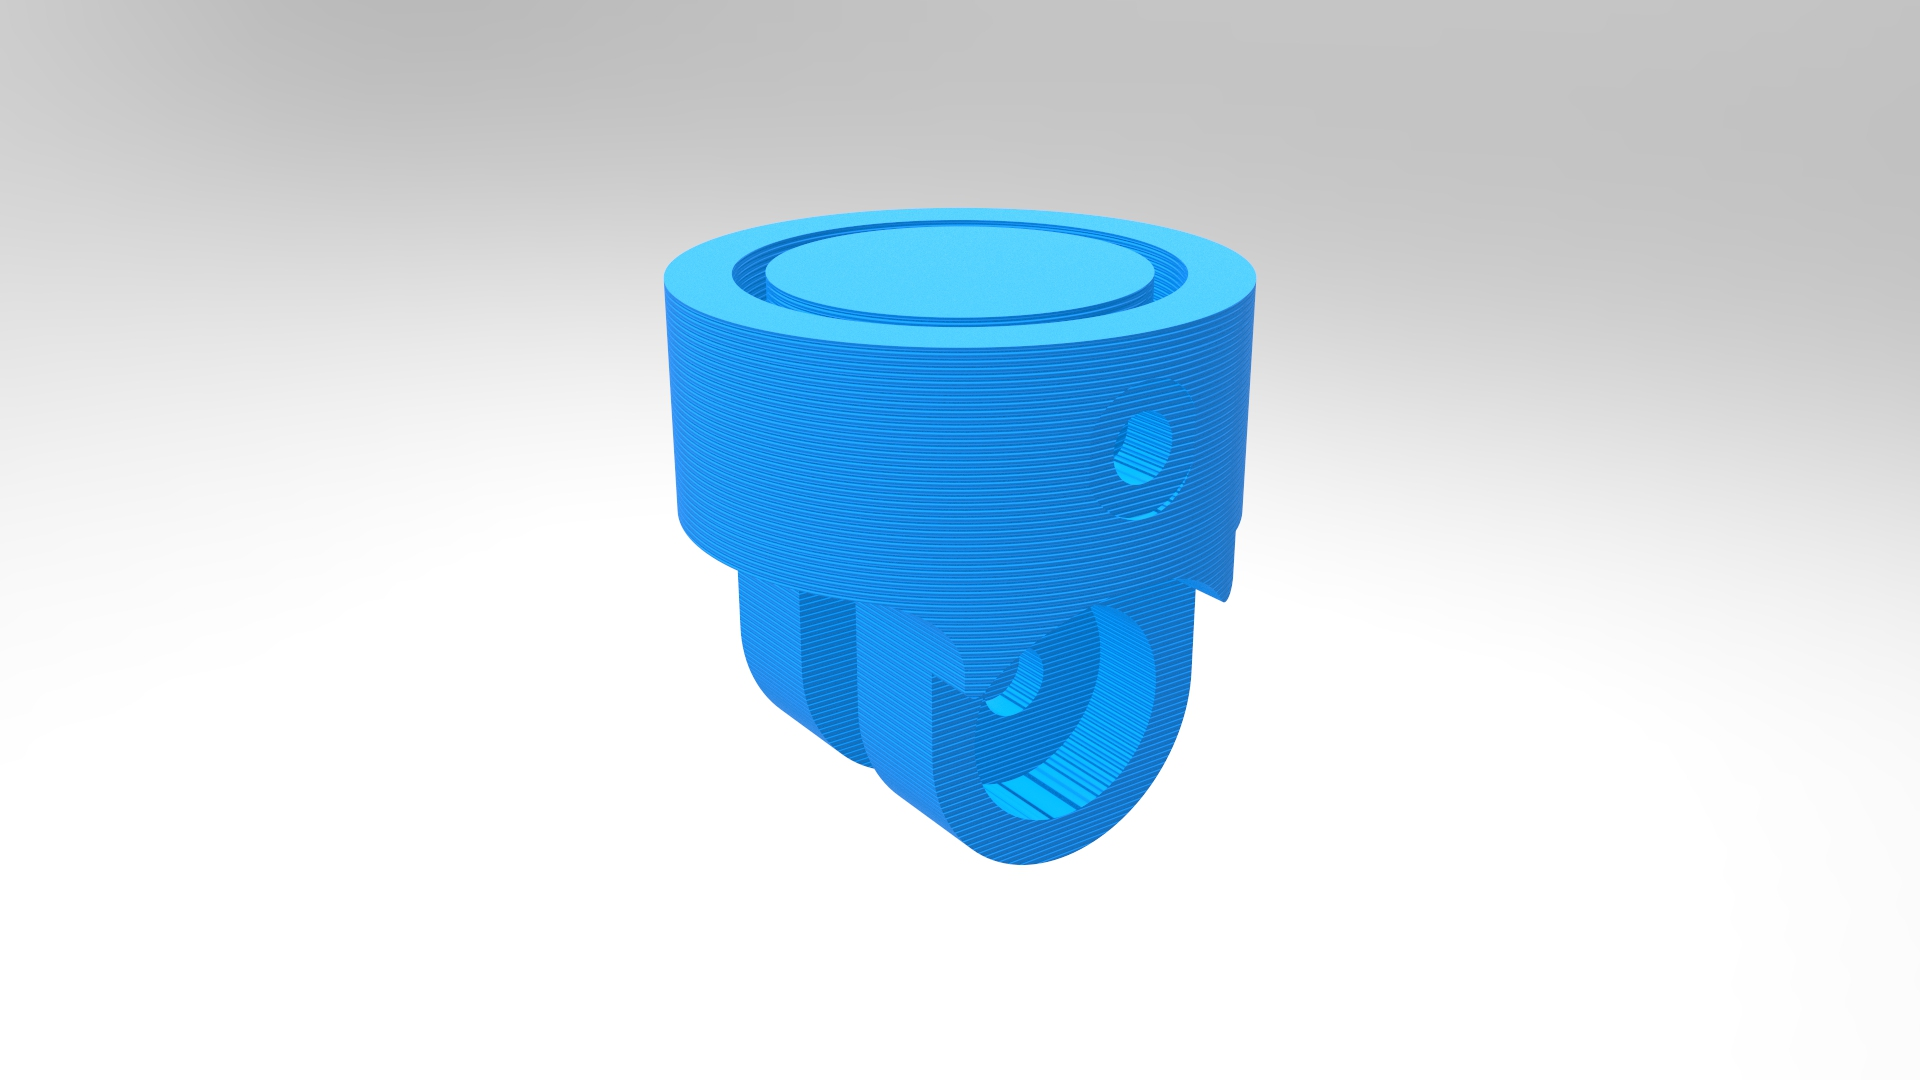
\includegraphics[width=\textwidth]{figures/legs_ankle_upper.jpg}
        \caption{Left upper ankle}
        \label{fig:ankle_upper}
    \end{subfigure}
    \begin{subfigure}[b]{0.49\textwidth}
        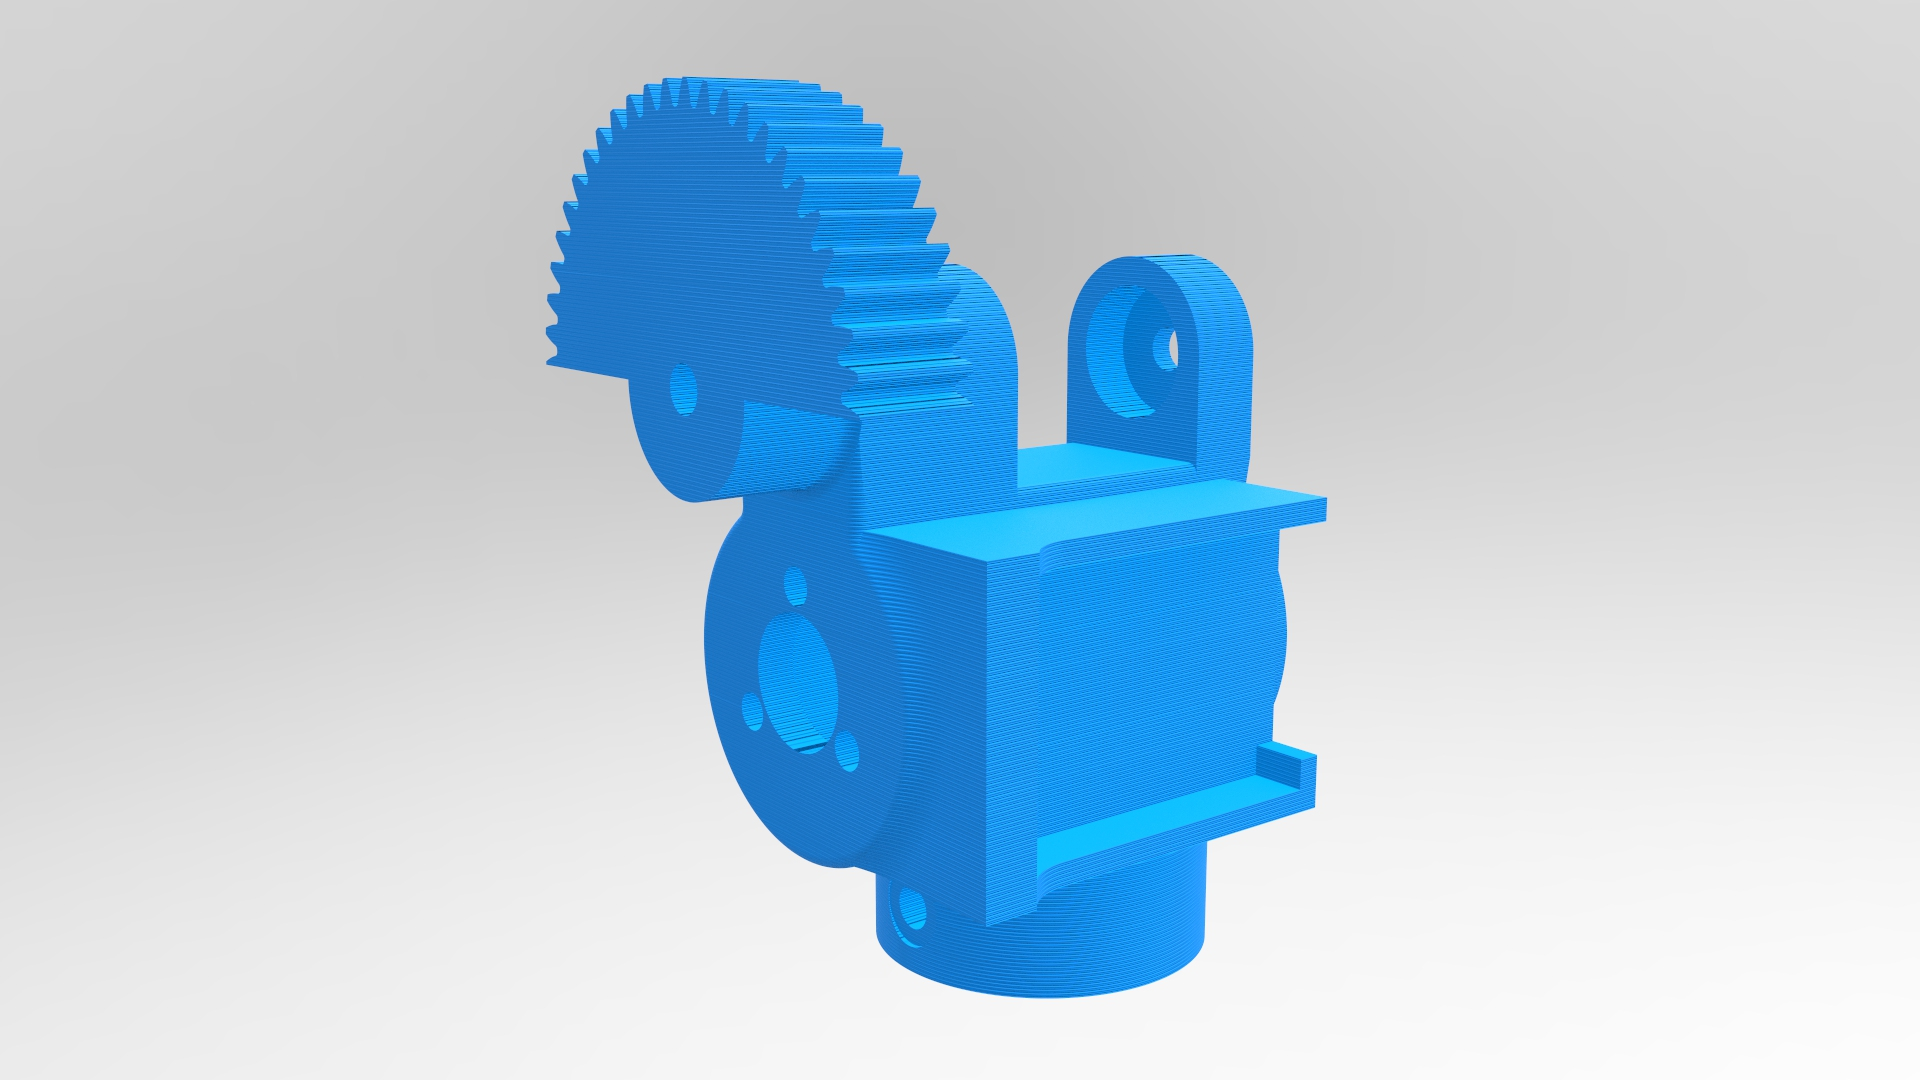
\includegraphics[width=\textwidth]{figures/legs_hip_lower.jpg}
        \caption{Left lower hip}
        \label{fig:hip_lower}
    \end{subfigure}

    \begin{subfigure}[b]{0.49\textwidth}
        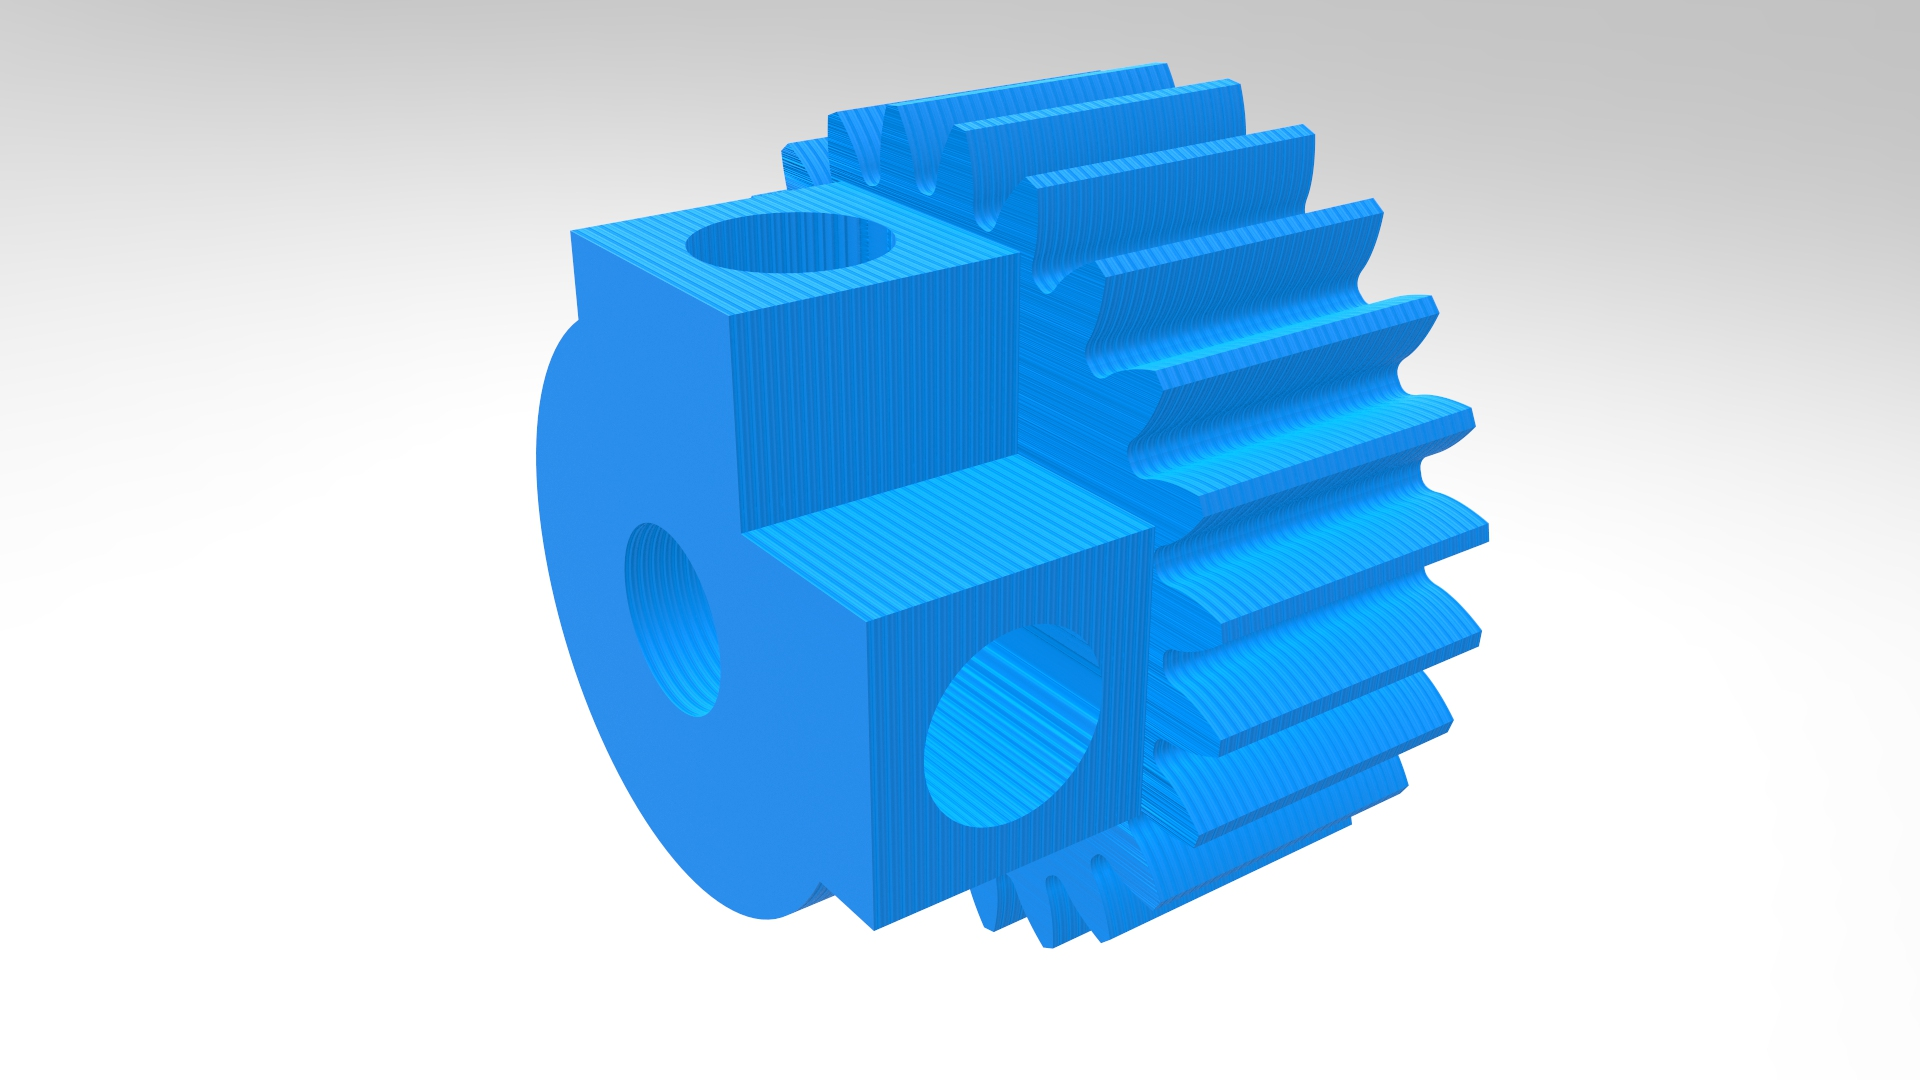
\includegraphics[width=\textwidth]{figures/legs_hip_pinion.jpg}
        \caption{Hip's pinion}
        \label{fig:hip_pinion}
    \end{subfigure}
    \begin{subfigure}[b]{0.49\textwidth}
        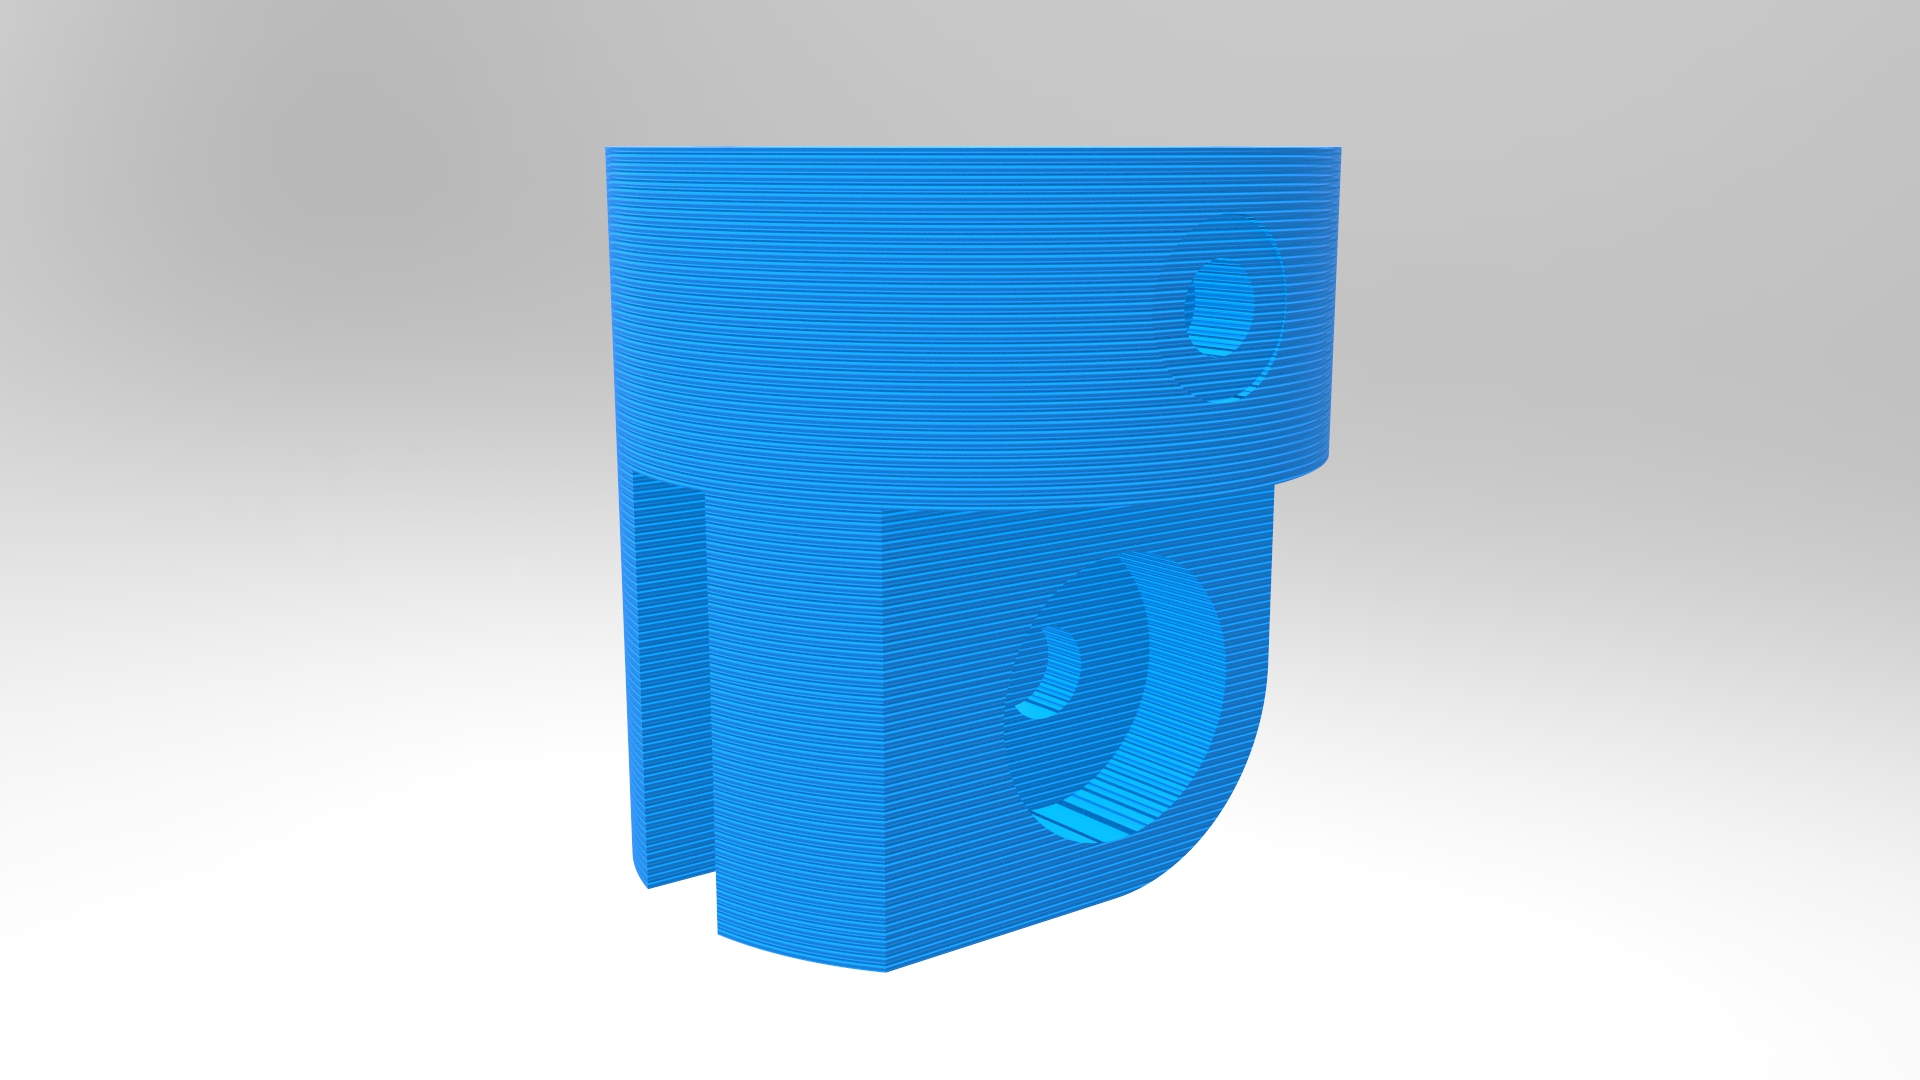
\includegraphics[width=\textwidth]{figures/legs_knee_upper.jpg}
        \caption{Left upper knee}
        \label{fig:knee_upper}
    \end{subfigure}
\end{figure}

% subsection computer_aided_design (end)

% section mechanics (end)
%!TEX root = ../../../report.tex
\section{Software} % (fold)
\label{sec:software}

%!TEX root = ../../../../report.tex

\subsection{Motivation} % (fold)
\label{sub:motivation}
When approaching the task of designing a new robotic platform for the AI department at the Mærsk Mc-Kinney Møller Institute, the current development environment being utilized and its capabilities were studied as a first step.
Nowadays, the simulation and control of the robots at the department is based on the LPZrobots \cite{lpzrobots} and Gorobots \cite{gorobots} packages.
These software tools provide both a simulation engine for robots built on ODE \cite{ode}, OSG \cite{osg} and a framework for an easy implementation of controllers in both simulation and hardware.
However, their specificity compared to other existing instruments collides with some of the core design ideas of the robot framework presented here, which are simplicity of use and generalization.
The above mentioned are the reasons why it was decided to migrate the development environment to ROS Jade \cite{ros} for the bipedal locomotion study framework of RuBy. 

% subsection motivation (end)
%!TEX root = ../../../../report.tex

\subsection{ROS control} % (fold)
\label{sub:ros_control}

% subsection ros_control (end)
%!TEX root = ../../../../report.tex
\subsection{ROS Control-to-Hardware interface} % (fold)
\label{sub:ros_control_hardware_locokit_interface}
The Locokit embedded electronics comes along a standard C library called LocoAPI designed for an easy interaction and use of the capabilities of its hardware, as presented in \cite{locokit}.
This library has been utilized to implement the basic hardware functionalities in Rubi without any modification.
However, it can be easily edited or extended in order to add new ones if needed, which was considered a great advantage during the selection of the hardware platform.

The Locokit can be configured to offer a wireless interface between its main processor and an external computer creating and add-hoc WiFi network in the Gumstix.
Besides, it offers a ready-to-use $C$ application based on the LocoAPI to work as the server side when interfacing the hardware. \ref{} %add actuateMotors.c to code stack?
Its setup and use instructions can be found in the Locokit documentation, supplied with the kit.
This left the client side of the wireless connection as the one that needed to be created.
An existing client application built as an "AbstractController" for the LPZrobots framework was already available. 
However, as explained before, to eliminate any dependency with LPZrobots and in order to use it within ROS Control, it was rewritten as an instantiation of "RobotHW" making use of the LocoKitInterface and ConnectionClass $C++$ classes provided.

\subsubsection{The Locokit HW interface node} % (fold)
\label{ssub:the_locokit_hw_interface}
The resulting ROS node currently implements the functions listed in \ref{list:locoHW_functions}.
They are fully operative and have been tested before assembling the actuators to the joints.

\begin{itemize}
\label{list:locoHW_functions}
	\item Setup of wireless connection: connect to the TCP websocket created in the server side. It requires the IP and port on the server side.
	\item Registration of HW interface handlers for ROS Controller Manager: currently Effort commands and Joint State readings can be transmitted.
	\item Transmission of motor commands to motor boards in HW side: PWM signal values. It requires the physical addresses of all the motor boards connected.
	\item Reception of joint state readings from motor boards: encoder tics for relative position
	\item Real-time handling of information transfer from/to the Controller Manager
\end{itemize}

The node can be extended with new standard/customized HW interface handlers and more functions from the "LocokitInterface" class for future applications.
However, it lacks some capabilities that will be of relevance for an optimal functioning of the Rubi robot and that failed be implemented due to time constraints or lack of resources. 
The main ones are listed in \ref{list:locoHW_functions_left}.

\begin{itemize}
\label{list:locoHW_functions_left}
	\item An initialization of the encoders to a predefined position set as zero in order to compute absolute position values.
	\item A new data flow channel to manage the sensory feedback information from non-built-in sensors, at the ground contact switches.
	\item If necessary, a mapping between the Effort command values received from the controller and the valid PWM signals sent to the motors.  
\end{itemize}
% subsubsection the_locokit_hw_interface (end)

\todo{Add roslaunch explanation in rubi\_bringup package?}

% subsection ros_control_hardware_locokit_interface (end)
%!TEX root = ../../../../report.tex

\subsection{Example controllers} % (fold)
\label{sub:example_controllers}
From the \textit{Controller manager} from ROS Control, different joint controllers can be handled.
In the example controllers the position controller and the effort controllers are used individually for each joint.
This joint controllers offer then a topic (e.g. /rubi/left\_ankle\_position) that the user can use to move the actuators.
This are created from a unique package called \textit{rubi\_joint\_controllers}.
It is worth to say that the position controllers are implemented with a PID and that these values have been adjusted experimentally with the simulations for each joint.

Two type of controllers are given that show a different range of options to use with the robot are presented.
Both are gathered in a sole package called \textit{rubi\_controllers}, which gives a more tidy and resource-shared environment rather than having a package for each controller.
This also makes really easy to deploy a new controller by removing all the creation process of a new package.
In order to start a new piece of code this must be created and then added in the \textit{CMakeLists.txt} from where also some examples are included.

The presented code follows the ROS conventions and the code style is the \textit{Google style} offered by the clang-code-model.
This creates a congruent workspace supervised by a git repository.

\subsubsection{Two neuron controller} % (fold)
\label{ssub:two_neuron_controller}
This first example controller shows how to:
\begin{enumerate}
    \item Use GoRobots.
    \item Make use of dynamic reconfigure.
    \item Adapts its behavior depending on gazebo real time factor.
\end{enumerate}
For the first, an example of how to link C++ code from GoRobots is shown in the \textit{CMakeLists.txt}.
This system is easier and more powerful than the current \textit{Makefiles} currently used in GoRobots.
The Artificial Neuronal Network (ANN) library is used to create a bi-neuronal network that creates the CPG signals of the actuators.
Furthermore, the synaptic weights can be modified by making use of the ROS feature \textit{Dynamic Reconfigurable Parameters}.
These offer an interface in order to change, on the fly, the the values of the created parameters.
In the figure \ref{fig:rqt_interface}, an RQT workspace containing the CPG signals and the dynamic reconfigurable parameters modifiers is depicted.

\begin{figure}[tb]
    \centering
    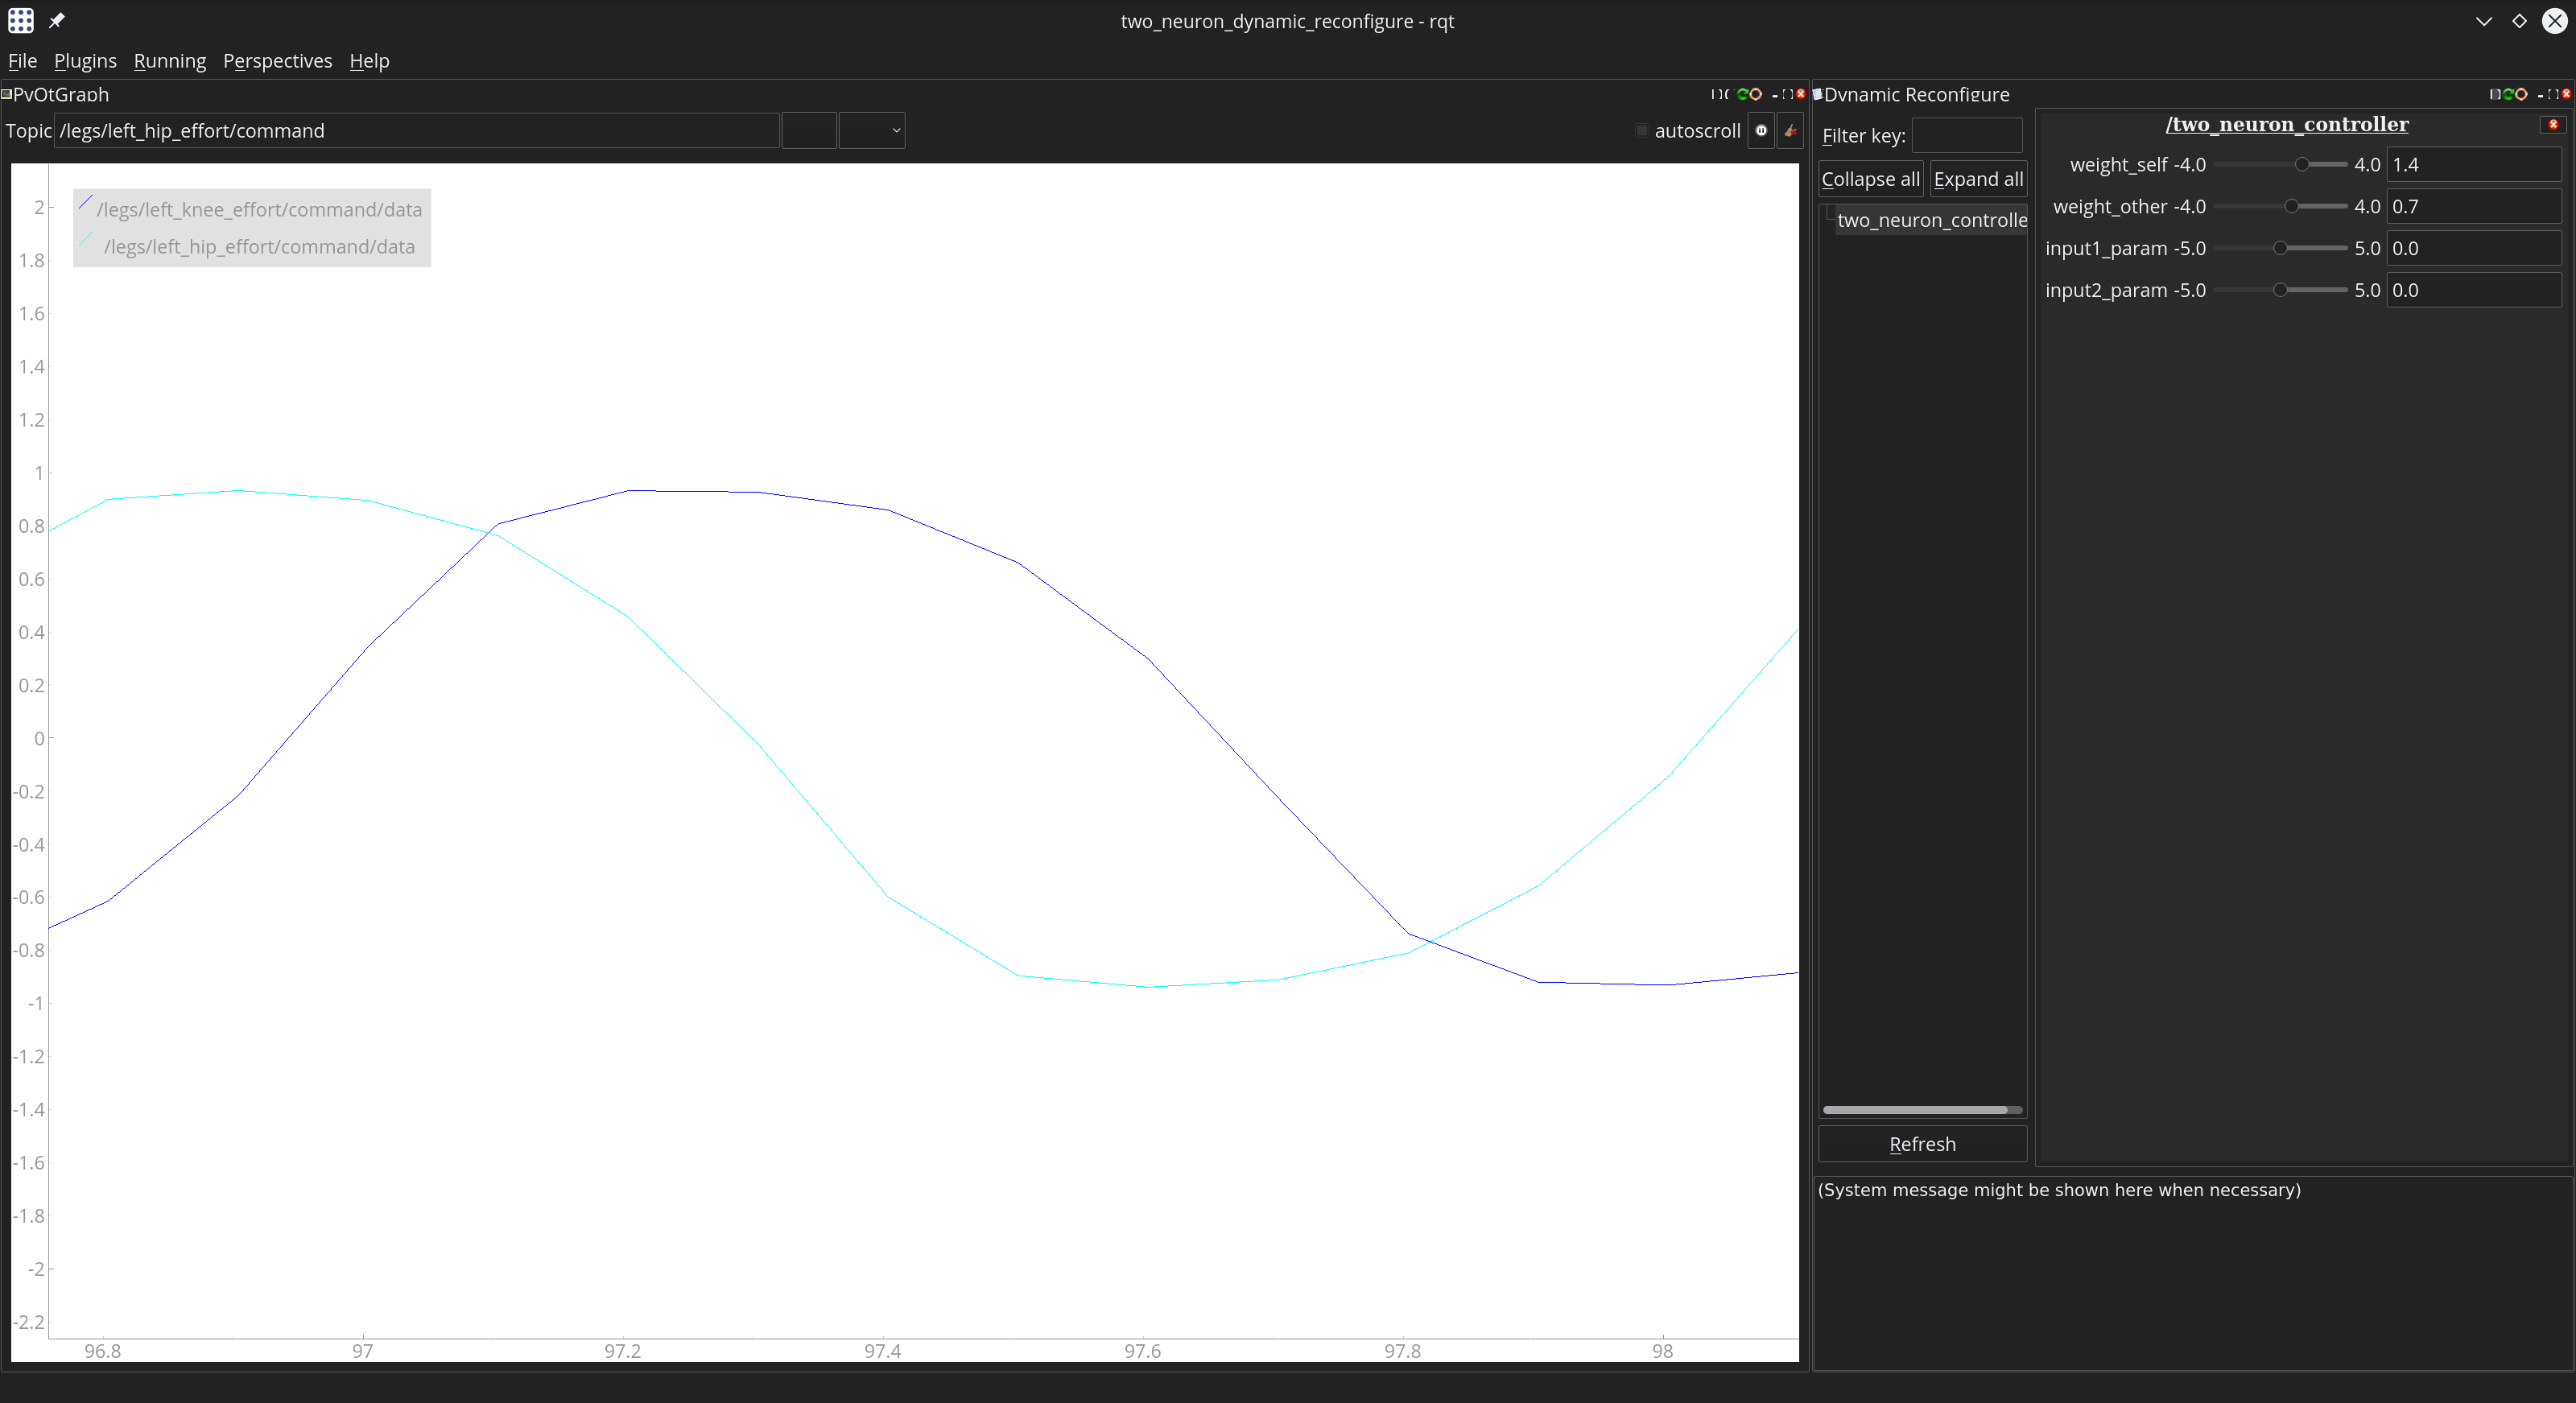
\includegraphics[width=\textwidth]{figures/rqt_interface}
    \caption{RQT workspace containing the CPG signals and the dynamic recofigurable parameters.}
    \label{fig:rqt_interface}
\end{figure}

This are also used to change the behavior of the ANN in order to be adapted to changes in Gazebo.
Gazebo uses can accelerate and decelerate the speed at which the time is passing through.
This is adjusted with a \textit{real time factor} that is read by the node and used to adjust the frequencies of the CPGs.
% subsubsection two_neuron_controller (end)

\subsubsection{Impulse controller} % (fold)
\label{ssub:impulse_controller}
Among other things this node shows how to:
\begin{enumerate}
    \item Load and unload different joint controllers.
    \item Give some wrappings for set of controllers (hoping position).
    \item Offer services for jumping: given a file or given the values and impulse time.
\end{enumerate}
This node implements some methods that enable it to change on-the-fly the controllers of each individual joint.
Furthermore, three combinations of individual joint controllers are given being these: (1) all in position mode, (2) all in effort mode and (3) left leg in position mode and right in effort mode.
The last one is useful when hoping, a moment in which a leg must hold a position and the other keep pushing in order to jump.

Three different services are implemented that impulse the robot in the sake of rise it from the floor.
The first two, are \textit{impulse\_one\_leg} and \textit{impulse\_two\_legs} which given a torque for each joint and an impulse time, it gives the possibility to jump either with one or two legs.
Both services load the necessary joint controllers in order to achieve the desired movements.
The third one offers sort of the same service but the parameters are read from a file instead.
This is handy when combined with the dynamic controller developed in MatLab and explained in the section \ref{sec_dynamic_model}.
% subsubsection impulse_controller (end)

% subsection example_controllers (end)

% section software (end)

% chapter design (end)chapters/cha_design/